\documentclass[12pt, a4paper]{article}

\usepackage[left=1cm,right=1cm,
    top=2cm,bottom=2cm, bindingoffset=0cm]{geometry}

\usepackage{cmap}
\usepackage[T2A]{fontenc}
\usepackage[utf8]{inputenc}
\usepackage[russian]{babel}

\usepackage[]{dot2texi}
\usepackage{tikz}
\usetikzlibrary{shapes,arrows}

\usepackage{amsmath, amsfonts}

\usepackage{float}

\title{Теоретические модели вычислений}
\title{ДЗ №1: Регулярные языки и конечные автоматы}
\author{Камила Гусамова, А-05-19}
\date{Март 2022}

%________________________________________________________________________________________________

\begin{document}
\maketitle

%________________________________________________________________________________________________

%часть 1%
\section{Задание №1. Построить конечный автомат, распознающий язык}%
Ответом на данное задание является конечный автомат, распознающий описанный язык. Автомат должен быть детерминированным.
\begin{enumerate}
%начало 1_1%
    \item \(L=\{\omega\in\{a,b,c\}^* | |\omega|_c = 1 \} \)
    
\begin{comment}
digraph {
    rankdir="LR"
    "" [shape=point]
    q1 [shape=circle]
    q2 [shape=doublecircle]
    
    "" -> q1
    q1 -> q1 [label="a,b"]
    q1 -> q2 [label="c"]
    q2 -> q2 [label="a,b"]
}
\end{comment}

    \begin{figure}[H]
        \centering
        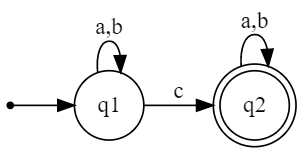
\includegraphics[scale=0.5]{1_1.png}
    \end{figure}
%конец 1_1%  
%начало 1_2%
    \item \(L=\{\omega\in\{a,b\}^* | |\omega|_a \leq 2, |\omega|_b \geq 2 \} \)
\\Рассмотрим \(L_1\) и \(L_2\) | \(L=L_1 \cap L_2\):
\\\(L_1=\{\omega\in\{a,b\}^* | |\omega|_a \leq 2 \} \)
\begin{comment}
digraph {
    rankdir="LR"
    "" [shape=point]
    q1 [shape=doublecircle]
    q2 [shape=doublecircle]
    q3 [shape=doublecircle]
    
    "" -> q1
    q1 -> q1 [label="b"]
    q1 -> q2 [label="a"]
    q2 -> q2 [label="b"]
    q2 -> q3 [label="a"]
    q3 -> q3 [label="b"]
}
\end{comment}

    \begin{figure}[H]
        \centering
        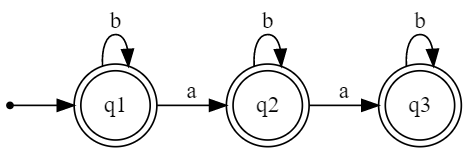
\includegraphics[scale=0.5]{1_2.png}
    \end{figure}
    
\(L_2=\{\omega\in\{a,b\}^* | |\omega|_b \geq 2 \} \)

\begin{comment}
digraph {
    rankdir="LR"
    "" [shape=point]
    q4 [shape=circle]
    q5 [shape=circle]
    q6 [shape=doublecircle]
    
    "" -> q4
    q4 -> q4 [label="a"]
    q4 -> q5 [label="b"]
    q5 -> q5 [label="a"]
    q5 -> q6 [label="b"]
    q6 -> q6 [label="a,b"]
}
\end{comment}

    \begin{figure}[H]
        \centering
        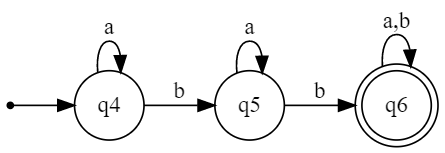
\includegraphics[scale=0.5]{1_3.png}
    \end{figure}
    
\(A_1=\{\Sigma_1=\{a,b\}, Q_1=\{q1,q2,q3\}, s_1=q1, T_1=\{q1,q2,q3\}, \delta_1\} \)
\\\(A_2=\{\Sigma_2=\{a,b\}, Q_2=\{q4,q5,q6\}, s_2=q4, T_2=\{q6\}, \delta_2\} \)
\\\(A=\{\Sigma, Q, s, T, \delta\} \):
\begin{itemize}
    \item \(\Sigma=\Sigma_1 \cup \Sigma_2=\{a,b\} \)
    \item \(Q=Q_1 \times Q_2=\{\langle q1,q4 \rangle, \langle q1,q5 \rangle, \langle q1,q6 \rangle, \langle q2,q4 \rangle, \langle q2,q5 \rangle, \langle q2,q6 \rangle, \langle q3,q4 \rangle, \langle q3,q5 \rangle, \langle q3,q6 \rangle\}\)
    \item \(s=\langle s1,s2 \rangle = \langle q1,q4 \rangle\)
    \item \(T=T_1 \times T_2=\langle q1,q6 \rangle, \langle q2,q6 \rangle, \langle q3,q6 \rangle\)
    \item \(\delta(\langle q_1,q_2 \rangle,c)=(\delta_1(q_1,c),\delta_2(q_2,c))\):
    \begin{itemize}
        \item \(\delta(\langle q1,q4 \rangle,a)=(\delta_1(q1,a),\delta_2(q4,a))=\langle q2,q4 \rangle\)
        \item \(\delta(\langle q1,q4 \rangle,b)=(\delta_1(q1,b),\delta_2(q4,b))=\langle q1,q5 \rangle\)
        \item \(\delta(\langle q1,q5 \rangle,a)=(\delta_1(q1,a),\delta_2(q5,a))=\langle q2,q5 \rangle\)
        \item \(\delta(\langle q1,q5 \rangle,b)=(\delta_1(q1,b),\delta_2(q5,b))=\langle q1,q6 \rangle\)
        \item \(\delta(\langle q1,q6 \rangle,a)=(\delta_1(q1,a),\delta_2(q6,a))=\langle q2,q6 \rangle\)
        \item \(\delta(\langle q1,q6 \rangle,b)=(\delta_1(q1,b),\delta_2(q6,b))=\langle q1,q6 \rangle\)
        
        \item \(\delta(\langle q2,q4 \rangle,a)=(\delta_1(q2,a),\delta_2(q4,a))=\langle q3,q4 \rangle\)
        \item \(\delta(\langle q2,q4 \rangle,b)=(\delta_1(q2,b),\delta_2(q4,b))=\langle q2,q5 \rangle\)
        \item \(\delta(\langle q2,q5 \rangle,a)=(\delta_1(q2,a),\delta_2(q5,a))=\langle q3,q5 \rangle\)
        \item \(\delta(\langle q2,q5 \rangle,b)=(\delta_1(q2,b),\delta_2(q5,b))=\langle q2,q6 \rangle\)
        \item \(\delta(\langle q2,q6 \rangle,a)=(\delta_1(q2,a),\delta_2(q6,a))=\langle q3,q6 \rangle\)
        \item \(\delta(\langle q2,q6 \rangle,b)=(\delta_1(q2,b),\delta_2(q6,b))=\langle q2,q6 \rangle\)
        
        \item \(\delta(\langle q3,q4 \rangle,a)=(\delta_1(q3,a),\delta_2(q4,a))=\emptyset\)
        \item \(\delta(\langle q3,q4 \rangle,b)=(\delta_1(q3,b),\delta_2(q4,b))=\langle q3,q5 \rangle\)
        \item \(\delta(\langle q3,q5 \rangle,a)=(\delta_1(q3,a),\delta_2(q5,a))=\emptyset\)
        \item \(\delta(\langle q3,q5 \rangle,b)=(\delta_1(q3,b),\delta_2(q5,b))=\langle q3,q6 \rangle\)
        \item \(\delta(\langle q3,q6 \rangle,a)=(\delta_1(q3,a),\delta_2(q6,a))=\emptyset\)
        \item \(\delta(\langle q3,q6 \rangle,b)=(\delta_1(q3,b),\delta_2(q6,b))=\langle q3,q6 \rangle\)
    \end{itemize}
\end{itemize}

\begin{comment}
digraph {
    rankdir="LR"
    "" [shape=point]
    q1q4 [shape=circle]
    q2q4 [shape=circle]
    q1q5 [shape=circle]
    q2q5 [shape=circle]
    q1q6 [shape=doublecircle]
    q2q6 [shape=doublecircle]
    q3q4 [shape=circle]
    q3q5 [shape=circle]
    q3q6 [shape=doublecircle]
    
    "" -> q1q4
    q1q4 -> q2q4 [label="a"]
    q1q4 -> q1q5 [label="b"]
    q1q5 -> q2q5 [label="a"]
    q1q5 -> q1q6 [label="b"]
    q1q6 -> q2q6 [label="a"]
    q1q6 -> q1q6 [label="b"]
    q2q4 -> q3q4 [label="a"]
    q2q4 -> q2q5 [label="b"]
    q2q5 -> q3q5 [label="a"]
    q2q5 -> q2q6 [label="b"]
    q2q6 -> q3q6 [label="a"]
    q2q6 -> q2q6 [label="b"]
    q3q4 -> q3q5 [label="b"]
    q3q5 -> q3q6 [label="b"]
    q3q6 -> q3q6 [label="b"]
} 
\end{comment}

    \begin{figure}[H]
        \centering
        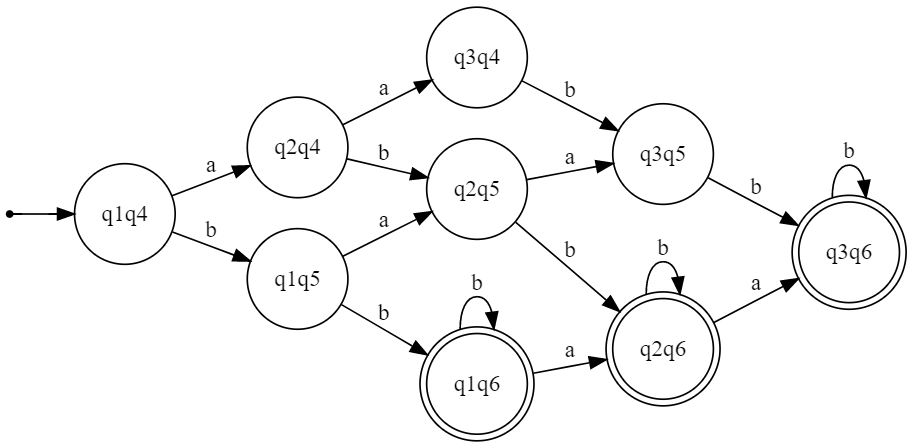
\includegraphics[width=0.6\columnwidth]{1_4.png}
    \end{figure}
%конец 1_2% 
%начало 1_3%
    \item \(L=\{\omega\in\{a,b\}^* | |\omega|_a \neq |\omega|_b \} \)
\\Построить ДКА, распознающий данный язык, невозможно, так как нам понадобится запоминать количество одинаковых символов -- это нельзя реализовать с помощью ДКА.
%конец 1_3%
%начало 1_4%
    \item \(L=\{\omega\in\{a,b\}^* | \omega\omega = \omega\omega\omega \} \)
\\Данному языку удовлетворяет только пустое слово:
\begin{comment}
digraph {
    rankdir="LR"
    "" [shape=point]
    q1 [shape=doublecircle]
    
    "" -> q1
} 
\end{comment}

    \begin{figure}[H]
        \centering
        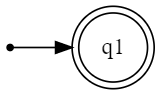
\includegraphics[scale=0.5]{1_5.png}
    \end{figure}
%конец 1_4%
\end{enumerate}

%________________________________________________________________________________________________

%часть 2%
\section{Задание №2. Построить конечный автомат, используя прямое произведение}%
Ответом на данное задание является конечный автомат, распознающий описанный язык. Требуется, чтобы он был построен при помощи прямого произведения ДКА и его свойств.

\begin{enumerate}
%начало 2_1%
    \item \(L_1=\{\omega\in\{a,b\}^* | |\omega|_a \geq 2 \wedge |\omega|_b \geq 2 \} \)
\(L_1=L_{11} \cap L_{12}\)
\\\(L_{11}=\{\omega\in\{a,b\}^* | |\omega|_a \geq 2 \} \)

\begin{comment}
digraph {
    rankdir="LR"
    "" [shape=point]
    q1 [shape=circle]
    q2 [shape=circle]
    q3 [shape=doublecircle]
    
    "" -> q1
    q1 -> q1 [label="b"]
    q1 -> q2 [label="a"]
    q2 -> q2 [label="b"]
    q2 -> q3 [label="a"]
    q3 -> q3 [label="a,b"]
}
\end{comment}

    \begin{figure}[H]
        \centering
        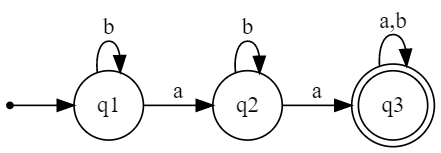
\includegraphics[scale=0.5]{2_1.png}
    \end{figure}
    
\(L_{12}=\{\omega\in\{a,b\}^* | |\omega|_b \geq 2 \} \)
\begin{comment}
digraph {
    rankdir="LR"
    "" [shape=point]
    q4 [shape=circle]
    q5 [shape=circle]
    q6 [shape=doublecircle]
    
    "" -> q4
    q4 -> q4 [label="a"]
    q4 -> q5 [label="b"]
    q5 -> q5 [label="a"]
    q5 -> q6 [label="b"]
    q6 -> q6 [label="a,b"]
}
\end{comment}

    \begin{figure}[H]
        \centering
        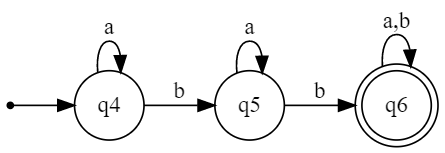
\includegraphics[scale=0.5]{2_2.png}
    \end{figure}

\(A_{11}=\{\Sigma_1=\{a,b\}, Q_1=\{q1,q2,q3\}, s_1=q1, T_1=\{q3\}, \delta_1\} \)
\\\(A_{12}=\{\Sigma_2=\{a,b\}, Q_2=\{q4,q5,q6\}, s_2=q4, T_2=\{q6\}, \delta_2\} \)
\\\(A_1=\{\Sigma, Q, s, T, \delta\} \):
\begin{itemize}
    \item \(\Sigma=\Sigma_1 \cup \Sigma_2=\{a,b\} \)
    \item \(Q=Q_1 \times Q_2=\{\langle q1,q4 \rangle, \langle q1,q5 \rangle, \langle q1,q6 \rangle, \langle q2,q4 \rangle, \langle q2,q5 \rangle, \langle q2,q6 \rangle, \langle q3,q4 \rangle, \langle q3,q5 \rangle, \langle q3,q6 \rangle\}\)
    \item \(s=\langle s1,s2 \rangle = \langle q1,q4 \rangle\)
    \item \(T=T_1 \times T_2= \langle q3,q6 \rangle\)
    \item \(\delta(\langle q_1,q_2 \rangle,c)=(\delta_1(q_1,c),\delta_2(q_2,c))\):
    \begin{itemize}
        \item \(\delta(\langle q1,q4 \rangle,a)=(\delta_1(q1,a),\delta_2(q4,a))=\langle q2,q4 \rangle\)
        \item \(\delta(\langle q1,q4 \rangle,b)=(\delta_1(q1,b),\delta_2(q4,b))=\langle q1,q5 \rangle\)
        \item \(\delta(\langle q1,q5 \rangle,a)=(\delta_1(q1,a),\delta_2(q5,a))=\langle q2,q5 \rangle\)
        \item \(\delta(\langle q1,q5 \rangle,b)=(\delta_1(q1,b),\delta_2(q5,b))=\langle q1,q6 \rangle\)
        \item \(\delta(\langle q1,q6 \rangle,a)=(\delta_1(q1,a),\delta_2(q6,a))=\langle q2,q6 \rangle\)
        \item \(\delta(\langle q1,q6 \rangle,b)=(\delta_1(q1,b),\delta_2(q6,b))=\langle q1,q6 \rangle\)
        
        \item \(\delta(\langle q2,q4 \rangle,a)=(\delta_1(q2,a),\delta_2(q4,a))=\langle q3,q4 \rangle\)
        \item \(\delta(\langle q2,q4 \rangle,b)=(\delta_1(q2,b),\delta_2(q4,b))=\langle q2,q5 \rangle\)
        \item \(\delta(\langle q2,q5 \rangle,a)=(\delta_1(q2,a),\delta_2(q5,a))=\langle q3,q5 \rangle\)
        \item \(\delta(\langle q2,q5 \rangle,b)=(\delta_1(q2,b),\delta_2(q5,b))=\langle q2,q6 \rangle\)
        \item \(\delta(\langle q2,q6 \rangle,a)=(\delta_1(q2,a),\delta_2(q6,a))=\langle q3,q6 \rangle\)
        \item \(\delta(\langle q2,q6 \rangle,b)=(\delta_1(q2,b),\delta_2(q6,b))=\langle q2,q6 \rangle\)
        
        \item \(\delta(\langle q3,q4 \rangle,a)=(\delta_1(q3,a),\delta_2(q4,a))=\langle q3,q4 \rangle\)
        \item \(\delta(\langle q3,q4 \rangle,b)=(\delta_1(q3,b),\delta_2(q4,b))=\langle q3,q5 \rangle\)
        \item \(\delta(\langle q3,q5 \rangle,a)=(\delta_1(q3,a),\delta_2(q5,a))=\langle q3,q5 \rangle\)
        \item \(\delta(\langle q3,q5 \rangle,b)=(\delta_1(q3,b),\delta_2(q5,b))=\langle q3,q6 \rangle\)
        \item \(\delta(\langle q3,q6 \rangle,a)=(\delta_1(q3,a),\delta_2(q6,a))=\langle q3,q6 \rangle\)
        \item \(\delta(\langle q3,q6 \rangle,b)=(\delta_1(q3,b),\delta_2(q6,b))=\langle q3,q6 \rangle\)
    \end{itemize}
\end{itemize}

\begin{comment}
digraph {
    rankdir="LR"
    "" [shape=point]
    q1q4 [shape=circle]
    q2q4 [shape=circle]
    q1q5 [shape=circle]
    q2q5 [shape=circle]
    q1q6 [shape=circle]
    q2q6 [shape=circle]
    q3q4 [shape=circle]
    q3q5 [shape=circle]
    q3q6 [shape=doublecircle]
    
    "" -> q1q4
    q1q4 -> q2q4 [label="a"]
    q1q4 -> q1q5 [label="b"]
    q1q5 -> q2q5 [label="a"]
    q1q5 -> q1q6 [label="b"]
    q1q6 -> q2q6 [label="a"]
    q1q6 -> q1q6 [label="b"]
    q2q4 -> q3q4 [label="a"]
    q2q4 -> q2q5 [label="b"]
    q2q5 -> q3q5 [label="a"]
    q2q5 -> q2q6 [label="b"]
    q2q6 -> q3q6 [label="a"]
    q2q6 -> q2q6 [label="b"]
    q3q4 -> q3q4 [label="a"]
    q3q4 -> q3q5 [label="b"]
    q3q5 -> q3q5 [label="a"]
    q3q5 -> q3q6 [label="b"]
    q3q6 -> q3q6 [label="a,b"]
} 
\end{comment}

    \begin{figure}[H]
        \centering
        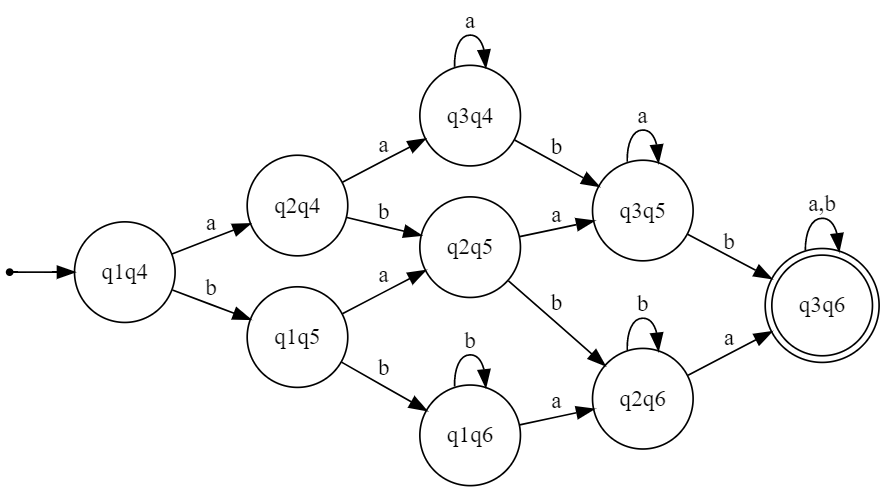
\includegraphics[width=0.6\columnwidth]{2_3.png}
    \end{figure}
%конец 2_1%
%начало 2_2%
    \item \(L_2=\{\omega \in\{a,b\}^* | |\omega| \geq 3 \wedge |\omega| \text{ нечётное} \} \)
\\\(L_2=L_{21} \cap L_{22}\)
\\\(L_{21}=\{\omega \in\{a,b\}^* | |\omega| \geq 3\} \)

\begin{comment}
digraph {
    rankdir="LR"
    "" [shape=point]
    q1 [shape=circle]
    q2 [shape=circle]
    q3 [shape=circle]
    q4 [shape=doublecircle]
    
    "" -> q1
    q1 -> q2 [label="a,b"]
    q2 -> q3 [label="a,b"]
    q3 -> q4 [label="a,b"]
    q4 -> q4 [label="a,b"]
}
\end{comment}

    \begin{figure}[H]
        \centering
        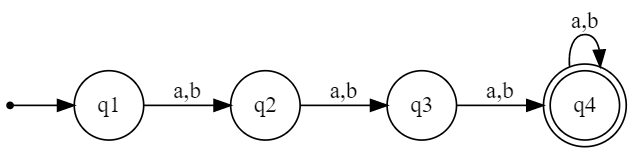
\includegraphics[width=0.6\columnwidth]{2_4.png}
    \end{figure}

\(L_{22}=\{\omega \in\{a,b\}^* | |\omega| \text{ нечётное} \} \)

\begin{comment}
digraph {
    rankdir="LR"
    "" [shape=point]
    q5 [shape=circle]
    q6 [shape=doublecircle]
    
    "" -> q5
    q5 -> q6 [label="a,b"]
    q6 -> q5 [label="a,b"]
}
\end{comment}

\(A_{21}=\{\Sigma_1=\{a,b\}, Q_1=\{q1,q2,q3,q4\}, s_1=q1, T_1=\{q4\}, \delta_1\} \)
\\\(A_{22}=\{\Sigma_2=\{a,b\}, Q_2=\{q5,q6\}, s_2=q5, T_2=\{q6\}, \delta_2\} \)
\\\(A_2=\{\Sigma, Q, s, T, \delta\} \):
\begin{itemize}
    \item \(\Sigma=\Sigma_1 \cup \Sigma_2=\{a,b\} \)
    \item \(Q=Q_1 \times Q_2=\{\langle q1,q5 \rangle, \langle q1,q6 \rangle, \langle q2,q5 \rangle, \langle q2,q6 \rangle, \langle q3,q5 \rangle, \langle q3,q6 \rangle, \langle q4,q5 \rangle, \langle q4,q6 \rangle\}\)
    \item \(s=\langle s1,s2 \rangle = \langle q1,q5 \rangle\)
    \item \(T=T_1 \times T_2= \langle q4,q6 \rangle\)
    \item \(\delta(\langle q_1,q_2 \rangle,c)=(\delta_1(q_1,c),\delta_2(q_2,c))\):
    \begin{itemize}
        \item \(\delta(\langle q1,q5 \rangle,a)=(\delta_1(q1,a),\delta_2(q5,a))=\langle q2,q6 \rangle\)
        \item \(\delta(\langle q1,q5 \rangle,b)=(\delta_1(q1,b),\delta_2(q5,b))=\langle q2,q6 \rangle\)
        \item \(\delta(\langle q1,q6 \rangle,a)=(\delta_1(q1,a),\delta_2(q6,a))=\langle q2,q5 \rangle\)
        \item \(\delta(\langle q1,q6 \rangle,b)=(\delta_1(q1,b),\delta_2(q6,b))=\langle q2,q5 \rangle\)
        
        \item \(\delta(\langle q2,q5 \rangle,a)=(\delta_1(q2,a),\delta_2(q5,a))=\langle q3,q6 \rangle\)
        \item \(\delta(\langle q2,q5 \rangle,b)=(\delta_1(q2,b),\delta_2(q5,b))=\langle q3,q6 \rangle\)
        \item \(\delta(\langle q2,q6 \rangle,a)=(\delta_1(q2,a),\delta_2(q6,a))=\langle q3,q5 \rangle\)
        \item \(\delta(\langle q2,q6 \rangle,b)=(\delta_1(q2,b),\delta_2(q6,b))=\langle q3,q5 \rangle\)
        
        \item \(\delta(\langle q3,q5 \rangle,a)=(\delta_1(q3,a),\delta_2(q5,a))=\langle q4,q6 \rangle\)
        \item \(\delta(\langle q3,q5 \rangle,b)=(\delta_1(q3,b),\delta_2(q5,b))=\langle q4,q6 \rangle\)
        \item \(\delta(\langle q3,q6 \rangle,a)=(\delta_1(q3,a),\delta_2(q6,a))=\langle q4,q5 \rangle\)
        \item \(\delta(\langle q3,q6 \rangle,b)=(\delta_1(q3,b),\delta_2(q6,b))=\langle q4,q5 \rangle\)
        
        \item \(\delta(\langle q4,q5 \rangle,a)=(\delta_1(q4,a),\delta_2(q5,a))=\langle q4,q6 \rangle\)
        \item \(\delta(\langle q4,q5 \rangle,b)=(\delta_1(q4,b),\delta_2(q5,b))=\langle q4,q6 \rangle\)
        \item \(\delta(\langle q4,q6 \rangle,a)=(\delta_1(q4,a),\delta_2(q6,a))=\langle q4,q5 \rangle\)
        \item \(\delta(\langle q4,q6 \rangle,b)=(\delta_1(q4,b),\delta_2(q6,b))=\langle q4,q5 \rangle\)
    \end{itemize}
\end{itemize}

\begin{comment}
digraph {
    rankdir="LR"
    "" [shape=point]
    q1q5 [shape=circle]
    q2q6 [shape=circle]
    q1q6 [shape=circle]
    q2q5 [shape=circle]
    q3q6 [shape=circle]
    q3q5 [shape=circle]
    q4q6 [shape=doublecircle]
    q4q5 [shape=circle]
    
    "" -> q1q5
    q1q5 -> q2q6 [label="a,b"]
    q1q6 -> q2q5 [label="a,b"]
    q2q5 -> q3q6 [label="a,b"]
    q2q6 -> q3q5 [label="a,b"]
    q3q5 -> q4q6 [label="a,b"]
    q3q6 -> q4q5 [label="a,b"]
    q4q5 -> q4q6 [label="a,b"]
    q4q6 -> q4q5 [label="a,b"]
}
\end{comment}

    \begin{figure}[H]
        \centering
        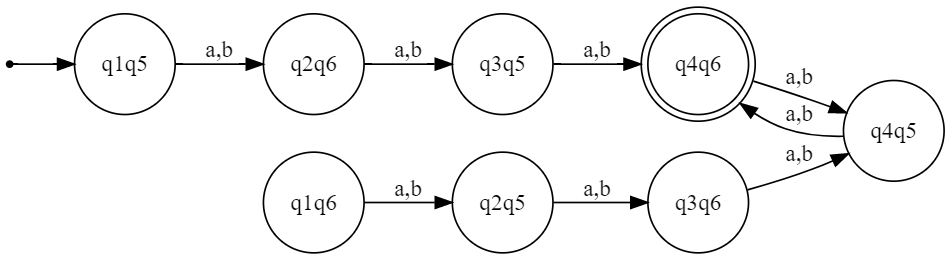
\includegraphics[width=0.6\columnwidth]{2_5.png}
    \end{figure}

\begin{comment}
digraph {
    rankdir="LR"
    "" [shape=point]
    q1q5 [shape=circle]
    q2q6 [shape=circle]
    q3q5 [shape=circle]
    q4q6 [shape=doublecircle]
    q4q5 [shape=circle]
    
    "" -> q1q5
    q1q5 -> q2q6 [label="a,b"]
    q2q6 -> q3q5 [label="a,b"]
    q3q5 -> q4q6 [label="a,b"]
    q4q5 -> q4q6 [label="a,b"]
    q4q6 -> q4q5 [label="a,b"]
}
\end{comment}

    \begin{figure}[H]
        \centering
        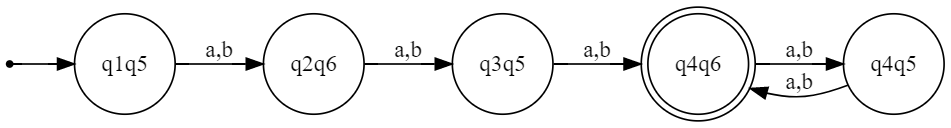
\includegraphics[width=0.6\columnwidth]{2_6.png}
    \end{figure}
%конец 2_2%
%начало 2_3%
    \item \(L_3=\{\omega\in\{a,b\}^* | |\omega|_a \text{ четно}\ \wedge |\omega|_b \text{ кратно трем} \} \)
\\\(L_3=L_{31} \cap L_{32}\)
\\\(L_{31}=\{\omega\in\{a,b\}^* | |\omega|_a \text{ четно}\ \} \)

\begin{comment}
digraph {
    rankdir="LR"
    "" [shape=point]
    q1 [shape=doublecircle]
    q2 [shape=circle]
    
    "" -> q1
    q1 -> q1 [label="b"]
    q1 -> q2 [label="a"]
    q2 -> q2 [label="b"]
    q2 -> q1 [label="a"]
}
\end{comment}

    \begin{figure}[H]
        \centering
        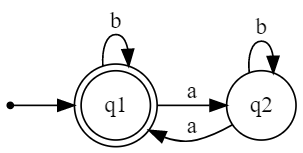
\includegraphics[scale=0.5]{2_7.png}
    \end{figure}

\(L_{32}=\{\omega\in\{a,b\}^* | |\omega|_b \text{ кратно трем} \} \)
\begin{comment}
digraph {
    rankdir="LR"
    "" [shape=point]
    q3 [shape=doublecircle]
    q4 [shape=circle]
    q5 [shape=circle]
    
    "" -> q3
    q3 -> q3 [label="a"]
    q3 -> q4 [label="b"]
    q4 -> q4 [label="a"]
    q4 -> q5 [label="b"]
    q5 -> q5 [label="a"]
    q5 -> q3 [label="b"]
}
\end{comment}

    \begin{figure}[H]
        \centering
        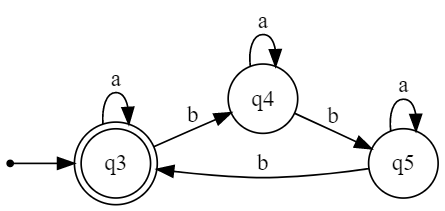
\includegraphics[scale=0.5]{2_8.png}
    \end{figure}

\(A_{31}=\{\Sigma_1=\{a,b\}, Q_1=\{q1,q2\}, s_1=q1, T_1=\{q1\}, \delta_1\} \)
\\\(A_{32}=\{\Sigma_2=\{a,b\}, Q_2=\{q3,q4,q5\}, s_2=q3, T_2=\{q3\}, \delta_2\} \)
\\\(A_3=\{\Sigma, Q, s, T, \delta\} \):
\begin{itemize}
    \item \(\Sigma=\Sigma_1 \cup \Sigma_2=\{a,b\} \)
    \item \(Q=Q_1 \times Q_2=\{\langle q1,q3 \rangle, \langle q1,q4 \rangle, \langle q1,q5 \rangle, \langle q2,q3 \rangle, \langle q2,q4 \rangle, \langle q2,q5 \rangle \}\)
    \item \(s=\langle s1,s2 \rangle = \langle q1,q3 \rangle\)
    \item \(T=T_1 \times T_2= \langle q1,q3 \rangle\)
    \item \(\delta(\langle q_1,q_2 \rangle,c)=(\delta_1(q_1,c),\delta_2(q_2,c))\):
    \begin{itemize}
        \item \(\delta(\langle q1,q3 \rangle,a)=(\delta_1(q1,a),\delta_2(q3,a))=\langle q2,q3 \rangle\)
        \item \(\delta(\langle q1,q3 \rangle,b)=(\delta_1(q1,b),\delta_2(q3,b))=\langle q1,q4 \rangle\)
        \item \(\delta(\langle q1,q4 \rangle,a)=(\delta_1(q1,a),\delta_2(q4,a))=\langle q2,q4 \rangle\)
        \item \(\delta(\langle q1,q4 \rangle,b)=(\delta_1(q1,b),\delta_2(q4,b))=\langle q1,q5 \rangle\)
        \item \(\delta(\langle q1,q5 \rangle,a)=(\delta_1(q1,a),\delta_2(q5,a))=\langle q2,q5 \rangle\)
        \item \(\delta(\langle q1,q5 \rangle,b)=(\delta_1(q1,b),\delta_2(q5,b))=\langle q1,q3 \rangle\)
        
        \item \(\delta(\langle q2,q3 \rangle,a)=(\delta_1(q2,a),\delta_2(q3,a))=\langle q1,q3 \rangle\)
        \item \(\delta(\langle q2,q3 \rangle,b)=(\delta_1(q2,b),\delta_2(q3,b))=\langle q2,q4 \rangle\)
        \item \(\delta(\langle q2,q4 \rangle,a)=(\delta_1(q2,a),\delta_2(q4,a))=\langle q1,q4 \rangle\)
        \item \(\delta(\langle q2,q4 \rangle,b)=(\delta_1(q2,b),\delta_2(q4,b))=\langle q2,q5 \rangle\)
        \item \(\delta(\langle q2,q5 \rangle,a)=(\delta_1(q2,a),\delta_2(q5,a))=\langle q1,q5 \rangle\)
        \item \(\delta(\langle q2,q5 \rangle,b)=(\delta_1(q2,b),\delta_2(q5,b))=\langle q2,q3 \rangle\)
    \end{itemize}
\end{itemize}

\begin{comment}
digraph {
    rankdir="LR"
    "" [shape=point]
    q1q3 [shape=doublecircle]
    q2q3 [shape=circle]
    q1q4 [shape=circle]
    q2q4 [shape=circle]
    q1q5 [shape=circle]
    q2q5 [shape=circle]
    
    "" -> q1q3
    q1q3 -> q2q3 [label="a"]
    q1q3 -> q1q4 [label="b"]
    q1q4 -> q2q4 [label="a"]
    q1q4 -> q1q5 [label="b"]
    q1q5 -> q2q5 [label="a"]
    q1q5 -> q1q3 [label="b"]
    q2q3 -> q1q3 [label="a"]
    q2q3 -> q2q4 [label="b"]
    q2q4 -> q1q4 [label="a"]
    q2q4 -> q2q5 [label="b"]
    q2q5 -> q1q5 [label="a"]
    q2q5 -> q2q3 [label="b"]
}
\end{comment}

    \begin{figure}[H]
        \centering
        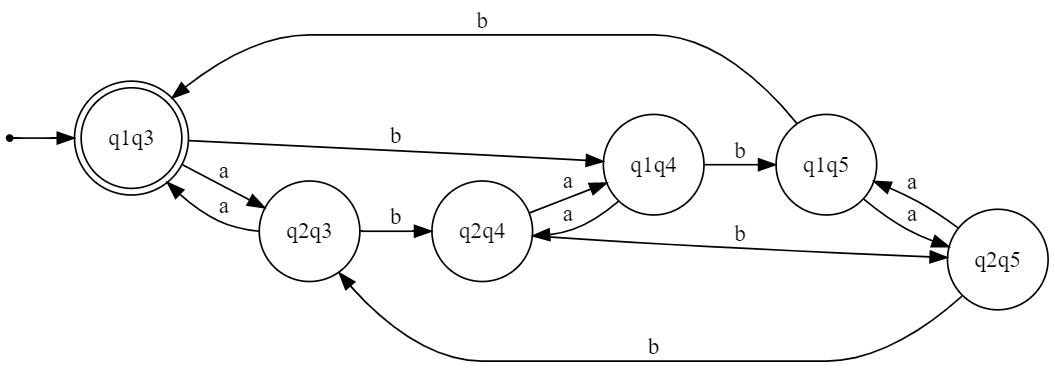
\includegraphics[width=0.6\columnwidth]{2_9.png}
    \end{figure}
%конец 2_3%
%начало 2_4%
    \item \(L_4=\overline{L_3}\)
\\\(L_4=\overline{L_3}=\{\Sigma_3, Q_3, s_3, T_3=Q_3 \setminus T_3, \delta_3\} \)
\\\(T_4=Q_3 \setminus T_3= \{\langle q1,q3 \rangle, \langle q1,q4 \rangle, \langle q1,q5 \rangle, \langle q2,q3 \rangle, \langle q2,q4 \rangle, \langle q2,q5 \rangle \} \setminus \{\langle q1,q3 \rangle\} = \{\langle q1,q4 \rangle, \langle q1,q5 \rangle, \langle q2,q3 \rangle, \langle q2,q4 \rangle, \langle q2,q5 \rangle \}\):

\begin{comment}
digraph {
    rankdir="LR"
    "" [shape=point]
    q1q3 [shape=circle]
    q2q3 [shape=doublecircle]
    q1q4 [shape=doublecircle]
    q2q4 [shape=doublecircle]
    q1q5 [shape=doublecircle]
    q2q5 [shape=doublecircle]
    
    "" -> q1q3
    q1q3 -> q2q3 [label="a"]
    q1q3 -> q1q4 [label="b"]
    q1q4 -> q2q4 [label="a"]
    q1q4 -> q1q5 [label="b"]
    q1q5 -> q2q5 [label="a"]
    q1q5 -> q1q3 [label="b"]
    q2q3 -> q1q3 [label="a"]
    q2q3 -> q2q4 [label="b"]
    q2q4 -> q1q4 [label="a"]
    q2q4 -> q2q5 [label="b"]
    q2q5 -> q1q5 [label="a"]
    q2q5 -> q2q3 [label="b"]
}
\end{comment}

    \begin{figure}[H]
        \centering
        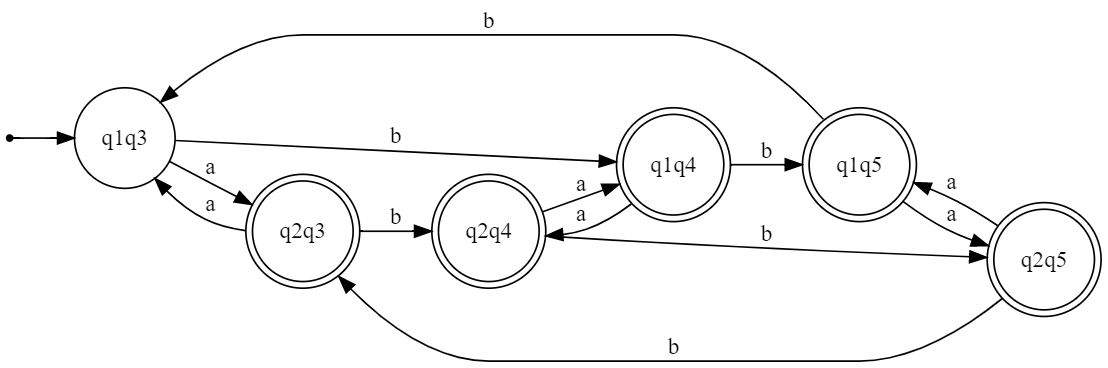
\includegraphics[width=0.6\columnwidth]{2_10.png}
    \end{figure}
    
    \item \(L_5=L_2 \setminus L_3\)
\\\(L_5=L_2 \setminus L_3=L_2 \cap \overline{L_3}\)
Для удобства переобозначим вершины автоматов, распознающих языки \(L_2\) и \(\overline{L_3}\):

\begin{comment}
digraph {
    rankdir="LR"
    "" [shape=point]
    Q1 [shape=circle]
    Q2 [shape=circle]
    Q3 [shape=circle]
    Q4 [shape=doublecircle]
    Q5 [shape=circle]
    
    "" -> Q1
    Q1 -> Q2 [label="a,b"]
    Q2 -> Q3 [label="a,b"]
    Q3 -> Q4 [label="a,b"]
    Q5 -> Q4 [label="a,b"]
    Q4 -> Q5 [label="a,b"]
}
\end{comment}

    \begin{figure}[H]
        \centering
        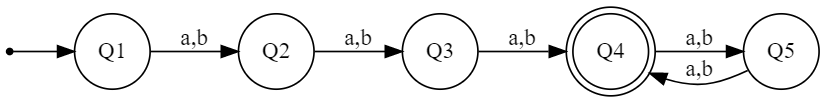
\includegraphics[width=0.6\columnwidth]{2_11.png}
    \end{figure}

\begin{comment}
digraph {
    rankdir="LR"
    "" [shape=point]
    Q6 [shape=circle]
    Q7 [shape=doublecircle]
    Q8 [shape=doublecircle]
    Q9 [shape=doublecircle]
    Q10 [shape=doublecircle]
    Q11 [shape=doublecircle]
    
    "" -> Q6
    Q6 -> Q7 [label="a"]
    Q6 -> Q8 [label="b"]
    Q8 -> Q9 [label="a"]
    Q8 -> Q10 [label="b"]
    Q10 -> Q11 [label="a"]
    Q10 -> Q6 [label="b"]
    Q7 -> Q6 [label="a"]
    Q7 -> Q9 [label="b"]
    Q9 -> Q8 [label="a"]
    Q9 -> Q11 [label="b"]
    Q11 -> Q10 [label="a"]
    Q11 -> Q7 [label="b"]
}
\end{comment}

    \begin{figure}[H]
        \centering
        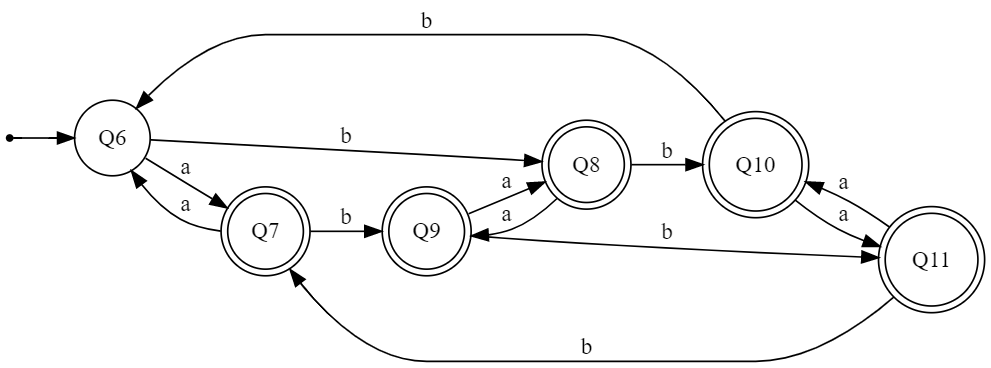
\includegraphics[width=0.6\columnwidth]{2_12.png}
    \end{figure}

\(A_3=\{\Sigma, Q, s, T, \delta\} \):
\begin{itemize}
    \item \(\Sigma=\Sigma_2 \cup \Sigma_{\overline{3}}=\{a,b\} \)
    \item \(Q=Q_2 \times Q_{\overline{3}}=\{\langle Q1,Q6 \rangle, \langle Q1,Q7 \rangle, \langle Q1,Q8 \rangle, \langle Q1,Q9 \rangle, \langle Q1,Q10 \rangle, \langle Q1,Q11 \rangle, \\\langle Q2,Q6 \rangle, \langle Q2,Q7 \rangle, \langle Q2,Q8 \rangle, \langle Q2,Q9 \rangle, \langle Q2,Q10 \rangle, \langle Q2,Q11 \rangle, \\\langle Q3,Q6 \rangle, \langle Q3,Q7 \rangle, \langle Q3,Q8 \rangle, \langle Q3,Q9 \rangle, \langle Q3,Q10 \rangle, \langle Q3,Q11 \rangle, \\\langle Q4,Q6 \rangle, \langle Q4,Q7 \rangle, \langle Q4,Q8 \rangle, \langle Q4,Q9 \rangle, \langle Q4,Q10 \rangle, \langle Q4,Q11 \rangle, \\\langle Q5,Q6 \rangle, \langle Q5,Q7 \rangle, \langle Q5,Q8 \rangle, \langle Q5,Q9 \rangle, \langle Q5,Q10 \rangle, \langle Q5,Q11 \rangle\}\)
    \item \(s=\langle s_2,s_{\overline{3}} \rangle = \langle Q1,Q6 \rangle\)
    \item \(T=T_2 \times T_{\overline{3}}= \langle Q4,Q7 \rangle, \langle Q4,Q8 \rangle, \langle Q4,Q9 \rangle, \langle Q4,Q10 \rangle, \langle Q4,Q11 \rangle\)
    \item \(\delta(\langle q_2,q_{\overline{3}} \rangle,c)=(\delta_1(q_2,c),\delta_2(q_{\overline{3}},c))\):
    \begin{itemize}
        \item \(\delta(\langle Q1,Q6 \rangle,a)=(\delta_1(Q1,a),\delta_2(Q6,a))=\langle Q2,Q7 \rangle\)
        \item \(\delta(\langle Q1,Q6 \rangle,b)=(\delta_1(Q1,b),\delta_2(Q6,b))=\langle Q2,Q8 \rangle\)
        \item \(\delta(\langle Q1,Q7 \rangle,a)=(\delta_1(Q1,a),\delta_2(Q7,a))=\langle Q2,Q6 \rangle\)
        \item \(\delta(\langle Q1,Q7 \rangle,b)=(\delta_1(Q1,b),\delta_2(Q7,b))=\langle Q2,Q9 \rangle\)
        \item \(\delta(\langle Q1,Q8 \rangle,a)=(\delta_1(Q1,a),\delta_2(Q8,a))=\langle Q2,Q9 \rangle\)
        \item \(\delta(\langle Q1,Q8 \rangle,b)=(\delta_1(Q1,b),\delta_2(Q8,b))=\langle Q2,Q10 \rangle\)
        \item \(\delta(\langle Q1,Q9 \rangle,a)=(\delta_1(Q1,a),\delta_2(Q9,a))=\langle Q2,Q8 \rangle\)
        \item \(\delta(\langle Q1,Q9 \rangle,b)=(\delta_1(Q1,b),\delta_2(Q9,b))=\langle Q2,Q11 \rangle\)
        \item \(\delta(\langle Q1,Q10 \rangle,a)=(\delta_1(Q1,a),\delta_2(Q10,a))=\langle Q2,Q11 \rangle\)
        \item \(\delta(\langle Q1,Q10 \rangle,b)=(\delta_1(Q1,b),\delta_2(Q10,b))=\langle Q2,Q6 \rangle\)
        \item \(\delta(\langle Q1,Q11 \rangle,a)=(\delta_1(Q1,a),\delta_2(Q11,a))=\langle Q2,Q10 \rangle\)
        \item \(\delta(\langle Q1,Q11 \rangle,b)=(\delta_1(Q1,b),\delta_2(Q11,b))=\langle Q2,Q7 \rangle\)
        
        \item \(\delta(\langle Q2,Q6 \rangle,a)=(\delta_1(Q2,a),\delta_2(Q6,a))=\langle Q3,Q7 \rangle\)
        \item \(\delta(\langle Q2,Q6 \rangle,b)=(\delta_1(Q2,b),\delta_2(Q6,b))=\langle Q3,Q8 \rangle\)
        \item \(\delta(\langle Q2,Q7 \rangle,a)=(\delta_1(Q2,a),\delta_2(Q7,a))=\langle Q3,Q6 \rangle\)
        \item \(\delta(\langle Q2,Q7 \rangle,b)=(\delta_1(Q2,b),\delta_2(Q7,b))=\langle Q3,Q9 \rangle\)
        \item \(\delta(\langle Q2,Q8 \rangle,a)=(\delta_1(Q2,a),\delta_2(Q8,a))=\langle Q3,Q9 \rangle\)
        \item \(\delta(\langle Q2,Q8 \rangle,b)=(\delta_1(Q2,b),\delta_2(Q8,b))=\langle Q3,Q10 \rangle\)
        \item \(\delta(\langle Q2,Q9 \rangle,a)=(\delta_1(Q2,a),\delta_2(Q9,a))=\langle Q3,Q8 \rangle\)
        \item \(\delta(\langle Q2,Q9 \rangle,b)=(\delta_1(Q2,b),\delta_2(Q9,b))=\langle Q3,Q11 \rangle\)
        \item \(\delta(\langle Q2,Q10 \rangle,a)=(\delta_1(Q2,a),\delta_2(Q10,a))=\langle Q3,Q11 \rangle\)
        \item \(\delta(\langle Q2,Q10 \rangle,b)=(\delta_1(Q2,b),\delta_2(Q10,b))=\langle Q3,Q6 \rangle\)
        \item \(\delta(\langle Q2,Q11 \rangle,a)=(\delta_1(Q2,a),\delta_2(Q11,a))=\langle Q3,Q10 \rangle\)
        \item \(\delta(\langle Q2,Q11 \rangle,b)=(\delta_1(Q2,b),\delta_2(Q11,b))=\langle Q3,Q7 \rangle\)
        
        \item \(\delta(\langle Q3,Q6 \rangle,a)=(\delta_1(Q3,a),\delta_2(Q6,a))=\langle Q4,Q7 \rangle\)
        \item \(\delta(\langle Q3,Q6 \rangle,b)=(\delta_1(Q3,b),\delta_2(Q6,b))=\langle Q4,Q8 \rangle\)
        \item \(\delta(\langle Q3,Q7 \rangle,a)=(\delta_1(Q3,a),\delta_2(Q7,a))=\langle Q4,Q6 \rangle\)
        \item \(\delta(\langle Q3,Q7 \rangle,b)=(\delta_1(Q3,b),\delta_2(Q7,b))=\langle Q4,Q9 \rangle\)
        \item \(\delta(\langle Q3,Q8 \rangle,a)=(\delta_1(Q3,a),\delta_2(Q8,a))=\langle Q4,Q9 \rangle\)
        \item \(\delta(\langle Q3,Q8 \rangle,b)=(\delta_1(Q3,b),\delta_2(Q8,b))=\langle Q4,Q10 \rangle\)
        \item \(\delta(\langle Q3,Q9 \rangle,a)=(\delta_1(Q3,a),\delta_2(Q9,a))=\langle Q4,Q8 \rangle\)
        \item \(\delta(\langle Q3,Q9 \rangle,b)=(\delta_1(Q3,b),\delta_2(Q9,b))=\langle Q4,Q11 \rangle\)
        \item \(\delta(\langle Q3,Q10 \rangle,a)=(\delta_1(Q3,a),\delta_2(Q10,a))=\langle Q4,Q11 \rangle\)
        \item \(\delta(\langle Q3,Q10 \rangle,b)=(\delta_1(Q3,b),\delta_2(Q10,b))=\langle Q4,Q6 \rangle\)
        \item \(\delta(\langle Q3,Q11 \rangle,a)=(\delta_1(Q3,a),\delta_2(Q11,a))=\langle Q4,Q10 \rangle\)
        \item \(\delta(\langle Q3,Q11 \rangle,b)=(\delta_1(Q3,b),\delta_2(Q11,b))=\langle Q4,Q7 \rangle\)
        
        \item \(\delta(\langle Q4,Q6 \rangle,a)=(\delta_1(Q4,a),\delta_2(Q6,a))=\langle Q5,Q7 \rangle\)
        \item \(\delta(\langle Q4,Q6 \rangle,b)=(\delta_1(Q4,b),\delta_2(Q6,b))=\langle Q5,Q8 \rangle\)
        \item \(\delta(\langle Q4,Q7 \rangle,a)=(\delta_1(Q4,a),\delta_2(Q7,a))=\langle Q5,Q6 \rangle\)
        \item \(\delta(\langle Q4,Q7 \rangle,b)=(\delta_1(Q4,b),\delta_2(Q7,b))=\langle Q5,Q9 \rangle\)
        \item \(\delta(\langle Q4,Q8 \rangle,a)=(\delta_1(Q4,a),\delta_2(Q8,a))=\langle Q5,Q9 \rangle\)
        \item \(\delta(\langle Q4,Q8 \rangle,b)=(\delta_1(Q4,b),\delta_2(Q8,b))=\langle Q5,Q10 \rangle\)
        \item \(\delta(\langle Q4,Q9 \rangle,a)=(\delta_1(Q4,a),\delta_2(Q9,a))=\langle Q5,Q8 \rangle\)
        \item \(\delta(\langle Q4,Q9 \rangle,b)=(\delta_1(Q4,b),\delta_2(Q9,b))=\langle Q5,Q11 \rangle\)
        \item \(\delta(\langle Q4,Q10 \rangle,a)=(\delta_1(Q4,a),\delta_2(Q10,a))=\langle Q5,Q11 \rangle\)
        \item \(\delta(\langle Q4,Q10 \rangle,b)=(\delta_1(Q4,b),\delta_2(Q10,b))=\langle Q5,Q6 \rangle\)
        \item \(\delta(\langle Q4,Q11 \rangle,a)=(\delta_1(Q4,a),\delta_2(Q11,a))=\langle Q5,Q10 \rangle\)
        \item \(\delta(\langle Q4,Q11 \rangle,b)=(\delta_1(Q4,b),\delta_2(Q11,b))=\langle Q5,Q7 \rangle\)
        
        \item \(\delta(\langle Q5,Q6 \rangle,a)=(\delta_1(Q5,a),\delta_2(Q6,a))=\langle Q4,Q7 \rangle\)
        \item \(\delta(\langle Q5,Q6 \rangle,b)=(\delta_1(Q5,b),\delta_2(Q6,b))=\langle Q4,Q8 \rangle\)
        \item \(\delta(\langle Q5,Q7 \rangle,a)=(\delta_1(Q5,a),\delta_2(Q7,a))=\langle Q4,Q6 \rangle\)
        \item \(\delta(\langle Q5,Q7 \rangle,b)=(\delta_1(Q5,b),\delta_2(Q7,b))=\langle Q4,Q9 \rangle\)
        \item \(\delta(\langle Q5,Q8 \rangle,a)=(\delta_1(Q5,a),\delta_2(Q8,a))=\langle Q4,Q9 \rangle\)
        \item \(\delta(\langle Q5,Q8 \rangle,b)=(\delta_1(Q5,b),\delta_2(Q8,b))=\langle Q4,Q10 \rangle\)
        \item \(\delta(\langle Q5,Q9 \rangle,a)=(\delta_1(Q5,a),\delta_2(Q9,a))=\langle Q4,Q8 \rangle\)
        \item \(\delta(\langle Q5,Q9 \rangle,b)=(\delta_1(Q5,b),\delta_2(Q9,b))=\langle Q4,Q11 \rangle\)
        \item \(\delta(\langle Q5,Q10 \rangle,a)=(\delta_1(Q5,a),\delta_2(Q10,a))=\langle Q4,Q11 \rangle\)
        \item \(\delta(\langle Q5,Q10 \rangle,b)=(\delta_1(Q5,b),\delta_2(Q10,b))=\langle Q4,Q6 \rangle\)
        \item \(\delta(\langle Q5,Q11 \rangle,a)=(\delta_1(Q5,a),\delta_2(Q11,a))=\langle Q4,Q10 \rangle\)
        \item \(\delta(\langle Q5,Q11 \rangle,b)=(\delta_1(Q5,b),\delta_2(Q11,b))=\langle Q4,Q7 \rangle\)
    \end{itemize}
\end{itemize}

\begin{comment}
digraph {
    rankdir="LR"
    "" [shape=point]
    Q1Q6 [shape=circle]
    Q2Q7 [shape=circle]
    Q2Q8 [shape=circle]
    Q1Q7 [shape=circle]
    Q2Q6 [shape=circle]
    Q2Q9 [shape=circle]
    Q1Q8 [shape=circle]
    Q2Q10 [shape=circle]
    Q1Q9 [shape=circle]
    Q2Q11 [shape=circle]
    Q1Q10 [shape=circle]
    Q1Q11 [shape=circle]
    Q3Q7 [shape=circle]
    Q3Q8 [shape=circle]
    Q3Q6 [shape=circle]
    Q3Q9 [shape=circle]
    Q3Q10 [shape=circle]
    Q3Q11 [shape=circle]
    Q4Q7 [shape=doublecircle]
    Q4Q8 [shape=doublecircle]
    Q4Q6 [shape=circle]
    Q4Q9 [shape=doublecircle]
    Q4Q10 [shape=circle]
    Q4Q11 [shape=doublecircle]
    Q5Q7 [shape=circle]
    Q5Q8 [shape=circle]
    Q5Q6 [shape=circle]
    Q5Q9 [shape=circle]
    Q5Q10 [shape=circle]
    Q5Q11 [shape=circle]
    
    "" -> Q1Q6
    Q1Q6 -> Q2Q7 [label="a"]
    Q1Q6 -> Q2Q8 [label="b"]
    Q1Q7 -> Q2Q6 [label="a"]
    Q1Q7 -> Q2Q9 [label="a"]
    Q1Q8 -> Q2Q9 [label="a"]
    Q1Q8 -> Q2Q10 [label="b"]
    Q1Q9 -> Q2Q8 [label="a"]
    Q1Q9 -> Q2Q11 [label="b"]
    Q1Q10 -> Q2Q11 [label="a"]
    Q1Q10 -> Q2Q6 [label="b"]
    Q1Q11 -> Q2Q10 [label="a"]
    Q1Q11 -> Q2Q7 [label="b"]
    Q2Q6 -> Q3Q7 [label="a"]
    Q2Q6 -> Q3Q8 [label="b"]
    Q2Q7 -> Q3Q6 [label="a"]
    Q2Q7 -> Q3Q9 [label="b"]
    Q2Q8 -> Q3Q9 [label="a"]
    Q2Q8 -> Q3Q10 [label="b"]
    Q2Q9 -> Q3Q8 [label="a"]
    Q2Q9 -> Q3Q11 [label="b"]
    Q2Q10 -> Q3Q11 [label="a"]
    Q2Q10 -> Q3Q6 [label="b"]
    Q2Q11 -> Q3Q10 [label="a"]
    Q2Q11 -> Q3Q7 [label="b"]
    Q3Q6 -> Q4Q7 [label="a"]
    Q3Q6 -> Q4Q8 [label="b"]
    Q3Q7 -> Q4Q6 [label="a"]
    Q3Q7 -> Q4Q9 [label="b"]
    Q3Q8 -> Q4Q9 [label="a"]
    Q3Q8 -> Q4Q10 [label="b"]
    Q3Q9 -> Q4Q8 [label="a"]
    Q3Q9 -> Q4Q11 [label="b"]
    Q3Q10 -> Q4Q11 [label="a"]
    Q3Q10 -> Q4Q6 [label="b"]
    Q3Q11 -> Q4Q10 [label="a"]
    Q3Q11 -> Q4Q7 [label="b"]
    Q4Q6 -> Q5Q7 [label="a"]
    Q4Q6 -> Q5Q8 [label="b"]
    Q4Q7 -> Q5Q6 [label="a"]
    Q4Q7 -> Q5Q9 [label="b"]
    Q4Q8 -> Q5Q9 [label="a"]
    Q4Q8 -> Q5Q10 [label="b"]
    Q4Q9 -> Q5Q8 [label="a"]
    Q4Q9 -> Q5Q11 [label="b"]
    Q4Q10 -> Q5Q11 [label="a"]
    Q4Q10 -> Q5Q6 [label="b"]
    Q4Q11 -> Q5Q10 [label="a"]
    Q4Q11 -> Q5Q7 [label="b"]
    Q5Q6 -> Q4Q7 [label="a"]
    Q5Q6 -> Q4Q8 [label="b"]
    Q5Q7 -> Q4Q6 [label="a"]
    Q5Q7 -> Q4Q9 [label="b"]
    Q5Q8 -> Q4Q9 [label="a"]
    Q5Q8 -> Q4Q10 [label="b"]
    Q5Q9 -> Q4Q8 [label="a"]
    Q5Q9 -> Q4Q11 [label="b"]
    Q5Q10 -> Q4Q11 [label="a"]
    Q5Q10 -> Q4Q6 [label="b"]
    Q5Q11 -> Q4Q10 [label="a"]
    Q5Q11 -> Q4Q7 [label="b"]
}
\end{comment}

    \begin{figure}[H]
        \centering
        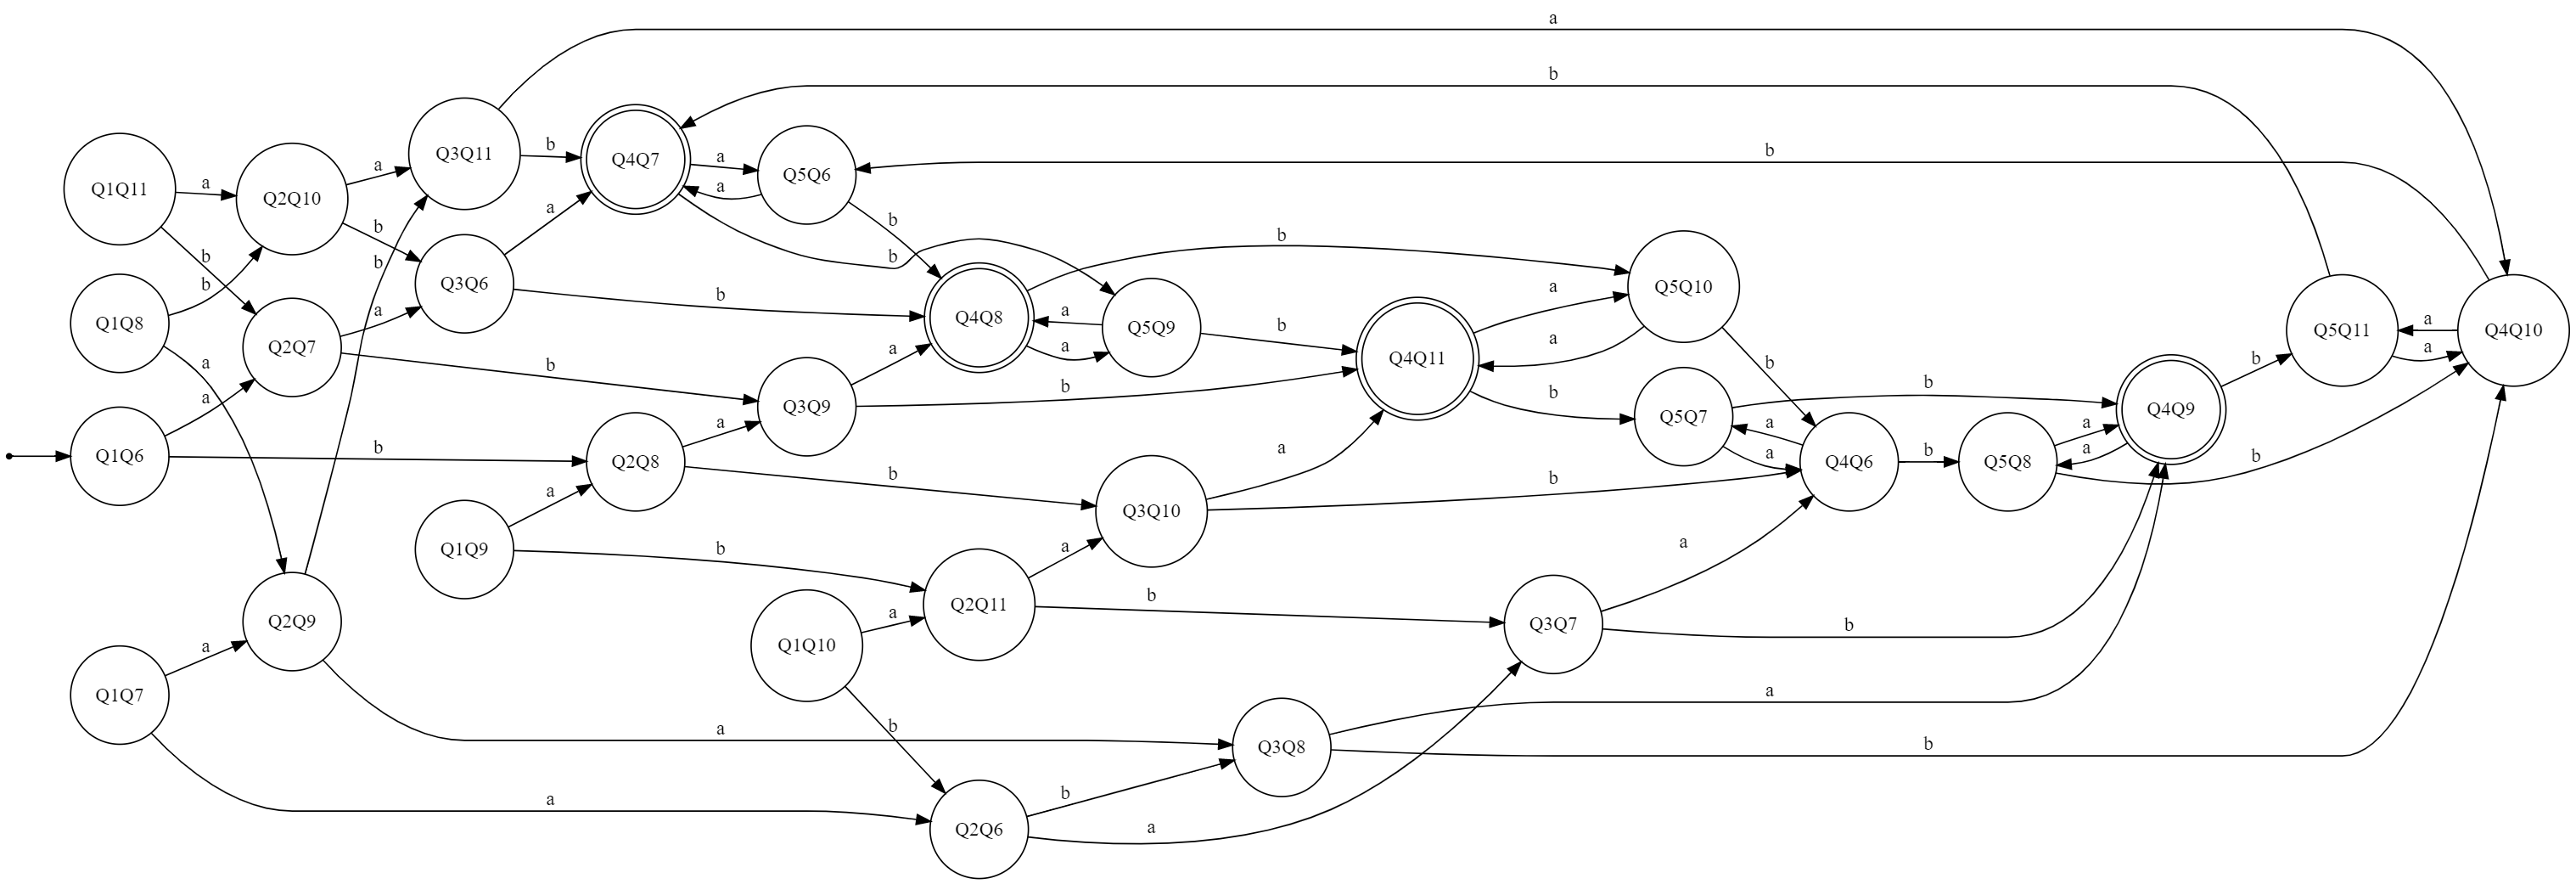
\includegraphics[width=1\columnwidth]{2_13.png}
    \end{figure}

\end{enumerate}
%\end{comment}

%часть 3%
\section{Задание №3. Построить минимальный ДКА по регулярному выражению.}
Ответом на данное задание является минимальный ДКА, который допускает тот же язык, что описывается регулярным выражением.
\\*Здесь мне уже не хватило сил на то, чтобы выписать все правила.
\begin{enumerate}
%начало 3_1%
    \item \((ab+aba)^*a\)
\\Строим НКА:
\begin{comment}
digraph {
    rankdir="LR"
    "" [shape=point]
    q1 [shape=circle]
    q2 [shape=circle]
    q3 [shape=circle]
    q4 [shape=circle]
    q5 [shape=circle]
    q6 [shape=circle]
    q7 [shape=circle]
    q8 [shape=circle]
    q9 [shape=circle]
    q10 [shape=circle]
    q11 [shape=circle]
    q12 [shape=doublecircle]

    "" -> q1 
    q1 -> q2 [label="λ"]
    q2 -> q3 [label="λ"]
    q3 -> q4 [label="a"]
    q4 -> q5 [label="b"]
    q5 -> q6 [label="λ"]
    q2 -> q7 [label="λ"]
    q7 -> q8 [label="a"]
    q8 -> q9 [label="b"]
    q9 -> q10 [label="a"]
    q10 -> q6 [label="λ"]
    q6 -> q11 [label="λ"]
    q11 -> q12 [label="a"]
    q6 -> q2 [label="λ"]
    q1 -> q11 [label="λ"]
}
\end{comment}
    \begin{figure}[H]
        \centering
        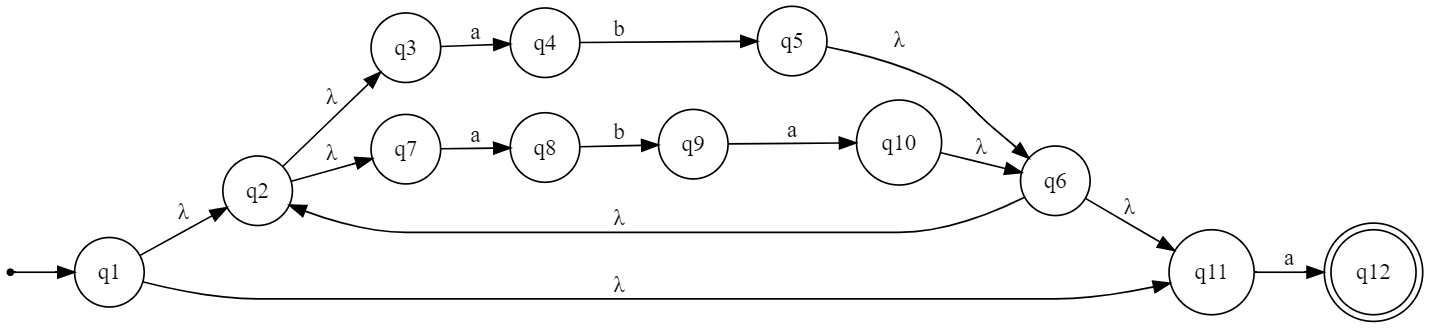
\includegraphics[width=0.6\columnwidth]{3_1.png}
    \end{figure}
Минимизируем \(\lambda\) и получим:
\begin{comment}
digraph {
    rankdir="LR"
    "" [shape=point]
    q1 [shape=circle]
    q2 [shape=circle]
    q3 [shape=circle]
    q4 [shape=circle]
    q5 [shape=circle]
    q6 [shape=circle]
    q7 [shape=circle]
    q8 [shape=circle]
    q9 [shape=circle]
    q10 [shape=doublecircle]

    "" -> q1 
    q1 -> q2 [label="λ"]
    q2 -> q3 [label="a"]
    q3 -> q4 [label="b"]
    q4 -> q5 [label="λ"]
    q1 -> q6 [label="λ"]
    q6 -> q7 [label="a"]
    q7 -> q8 [label="b"]
    q8 -> q9 [label="a"]
    q9 -> q5 [label="λ"]
    q5 -> q10 [label="a"]
    q5 -> q1 [label="λ"]
    q1 -> q5 [label="λ"]
}
\end{comment}
    \begin{figure}[H]
        \centering
        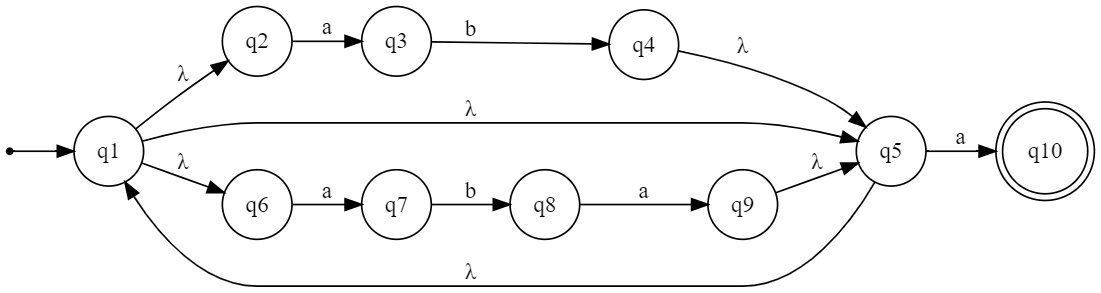
\includegraphics[width=0.6\columnwidth]{3_2.png}
    \end{figure}
    
Преобразуем в ДКА:

\begin{comment}
digraph {
    rankdir="LR"
    "" [shape=point]
    "{q1q2q5q9}" [shape=circle]
    "{q3,q7,q10}" [shape=doublecircle]
    "{q4q8}" [shape=circle]
    "{q3,q7,q9,q10}" [shape=doublecircle]

    "" -> "{q1q2q5q9}"
    "{q1q2q5q9}" -> "{q3,q7,q10}" [label="a"]
    "{q3,q7,q10}" -> "{q4q8}" [label="b"]
    "{q4q8}" -> "{q3,q7,q9,q10}" [label="a"]
    "{q3,q7,q9,q10}" -> "{q4q8}" [label="b"]
    "{q3,q7,q9,q10}" -> "{q3,q7,q10}" [label="a"]
}
\end{comment}
    \begin{figure}[H]
        \centering
        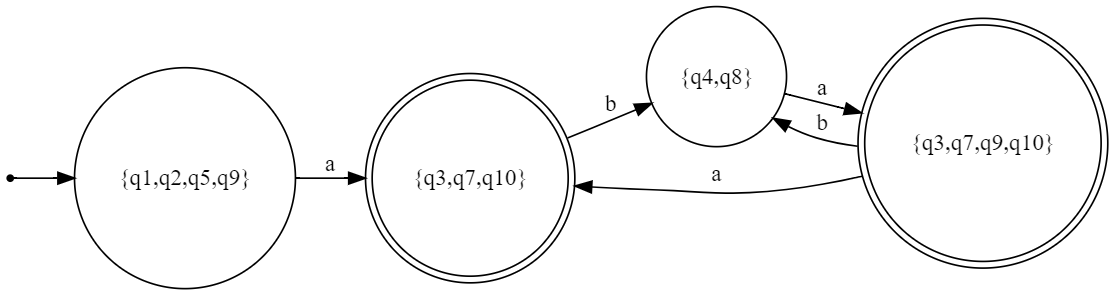
\includegraphics[width=0.6\columnwidth]{3_3.png}
    \end{figure}
    
Данный ДКА уже является минимальным.
%конец 3_1%

%начало 3_2%
    \item \(a(a(ab)^*b)(ab)^*\)
\\Строим НКА:
\begin{comment}
digraph {
    rankdir="LR"
    "" [shape=point]
    q1 [shape=circle]
    q2 [shape=circle]
    q3 [shape=circle]
    q4 [shape=circle]
    q5 [shape=circle]
    q6 [shape=doublecircle]
    q7 [shape=circle]
    q8 [shape=doublecircle]

    "" -> q1
    q1 -> q2 [label="a"]
    q1 -> q8 [label="a"]
    q2 -> q3 [label="a"]
    q3 -> q4 [label="a"]
    q3 -> q6 [label="b"]
    q4 -> q5 [label="b"]
    q5 -> q4 [label="a"]
    q5 -> q6 [label="b"]
    q6 -> q7 [label="a"]
    q7 -> q8 [label="b"]
    q8 -> q7 [label="a"]
}
\end{comment}

    \begin{figure}[H]
        \centering
        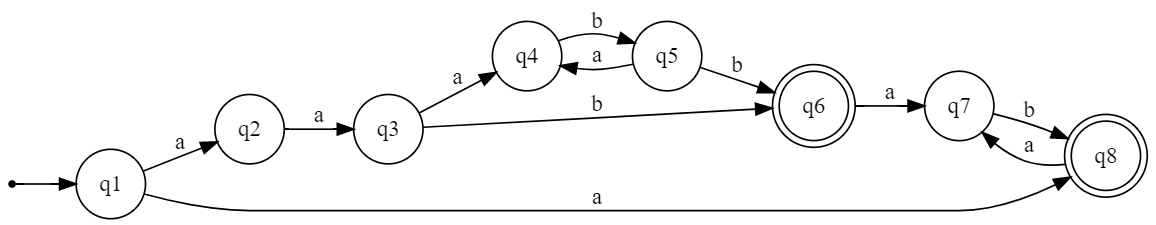
\includegraphics[width=0.6\columnwidth]{3_4.png}
    \end{figure}
    
Преобразуем в ДКА:

\begin{comment}
digraph {
    rankdir="LR"
    "" [shape=point]
    q1 [shape=circle]
    "{q2q8}" [shape=doublecircle]
    "{q3q7}" [shape=circle]
    "{q6q8}" [shape=doublecircle]
    q4 [shape=circle]
    q5 [shape=circle]
    q6 [shape=doublecircle]

    "" -> q1
    q1 -> "{q2q8}" [label="a"]
    "{q2q8}" -> "{q3q7}" [label="a"]
    "{q3q7}" -> q4 [label="a"]
    "{q3q7}" -> "{q6q8}" [label="b"]
    q4 -> q5 [label="b"]
    q5 -> q4 [label="a"]
    q5 -> q6 [label="b"]
    q6 -> "{q3q7}" [label="a"]
    "{q3q7}" -> "{q6q8}" [label="b"]
    "{q6q8}" -> "{q3q7}"
}
\end{comment}

    \begin{figure}[H]
        \centering
        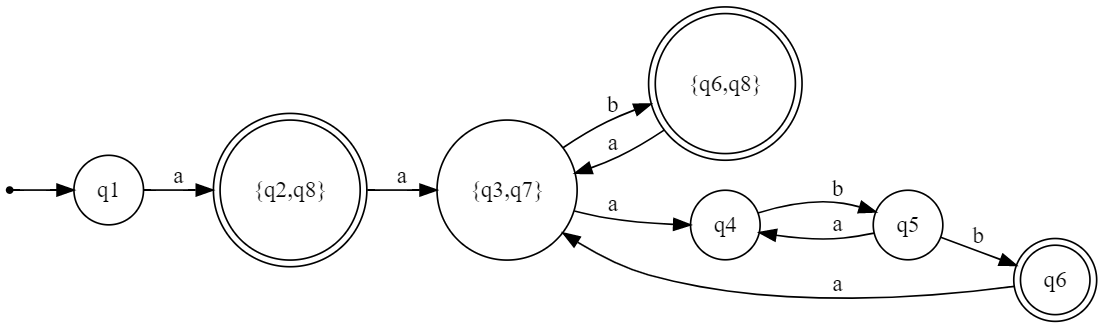
\includegraphics[width=0.6\columnwidth]{3_12.png}
    \end{figure}

Минимизируем его:

\begin{comment}
digraph {
    rankdir="LR"
    "" [shape=point]
    q1 [shape=circle]
    "{q6q8, q2q8, q6}" [shape=doublecircle]
    "q3q7, q5" [shape=circle]
    q4 [shape=circle]

    "" -> q1
    q1 -> "{q6q8, q2q8, q6}"  [label="a"]
    "{q6q8, q2q8, q6}" -> "q3q7, q5" [label="a"]
    "q3q7, q5" -> "{q6q8, q2q8, q6}" [label="b"]
    "q3q7, q5" -> q4 [label="a"]
    q4 -> "q3q7, q5" [label="b"]
}
\end{comment}

    \begin{figure}[H]
        \centering
        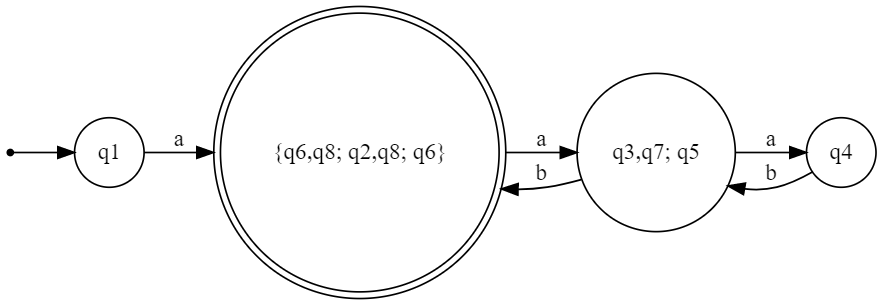
\includegraphics[width=0.6\columnwidth]{3_13.png}
    \end{figure}

%конец 3_2%

%начало 3_3%
    \item \((a+(a+b)(a+b)b)^*\)
    
\begin{comment}
digraph {
    rankdir="LR"
    "" [shape=point]
    q1 [shape=doublecircle]
    q2 [shape=circle]
    q3 [shape=circle]

    "" -> q1
    q1 -> q1 [label="a"]
    q1 -> q2 [label="a,b"]
    q2 -> q3 [label="a,b"]
    q3 -> q1 [label="b"]
}
\end{comment}

Строим НКА:

    \begin{figure}[H]
        \centering
        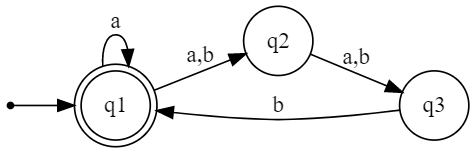
\includegraphics[scale=0.5]{3_5.png}
    \end{figure}
    
Преобразуем в ДКА:

\begin{comment}
digraph {
    rankdir="LR"
    "" [shape=point]
    q1 [shape=doublecircle]
    "{q1q2}" [shape=doublecircle]
    q2 [shape=circle]
    "{q1,q2,q3}" [shape=doublecircle]
    "{q2,q3}" [shape=circle]
    "{q1q3}" [shape=doublecircle]
    q3 [shape=circle]

    "" -> q1
    q1 -> "{q1q2}" [label="a"]
    q1 -> q2 [label="b"]
    "{q1q2}" -> "{q1,q2,q3}" [label="a"]
    "{q1,q2,q3}" -> "{q1,q2,q3}" [label="a,b"]
    "{q1q2}" -> "{q2,q3}" [label="b"]
    "{q2,q3}" -> "{q1q3}" [label="b"]
    "{q2,q3}" -> q3 [label="a"]
    "{q1q3}" -> "{q1q2}" [label="a,b"]
    q2 -> q3 [label="a,b"]
    q3 -> q1 [label="b"]
}
\end{comment}

    \begin{figure}[H]
        \centering
        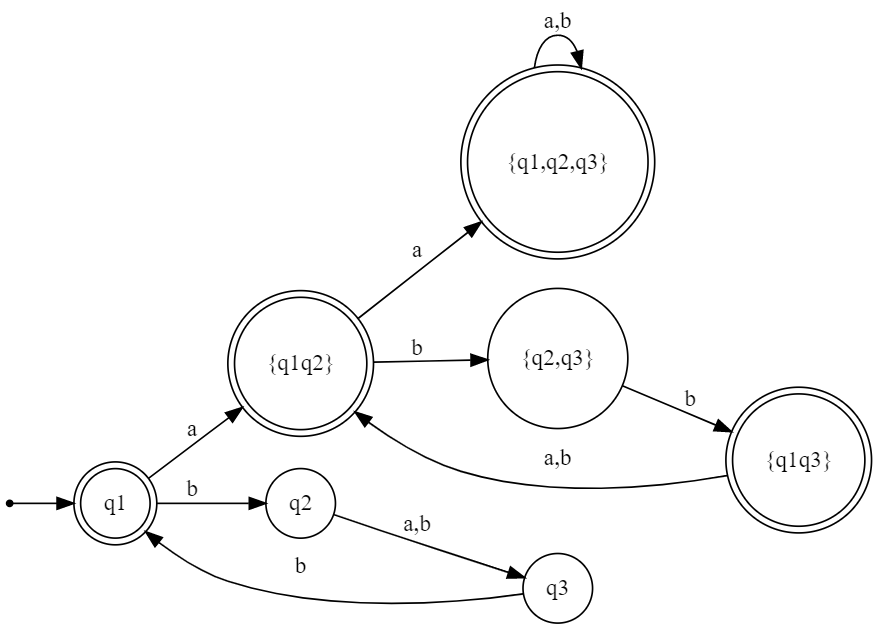
\includegraphics[width=0.6\columnwidth]{3_6.png}
    \end{figure}
    
Данный ДКА уже является минимальным.
%конец 3_3%

%начало 3_4%
    \item \((b+c)((ab)^*c+(ba)^*)^*\)
\\Построим ДКА:

\begin{comment}
digraph {
    rankdir="LR"
    "" [shape=point]
    q1 [shape=circle]
    q2 [shape=circle]
    q3 [shape=circle]
    q4 [shape=circle]
    q5 [shape=circle]
    q6 [shape=doublecircle]
    q7 [shape=doublecircle]

    "" -> q1
    q1 -> q2 [label="b,c"]
    q2 -> q3 [label="a"]
    q2 -> q4 [label="b"]
    q3 -> q5 [label="b"]
    q4 -> q6 [label="a"]
    q5 -> q3 [label="a"]
    q5 -> q7 [label="c"]
    q6 -> q4 [label="b"]
    q6 -> q3 [label="a"]
    q7 -> q3 [label="a"]
    q7 -> q4 [label="b"]
}
\end{comment}

    \begin{figure}[H]
        \centering
        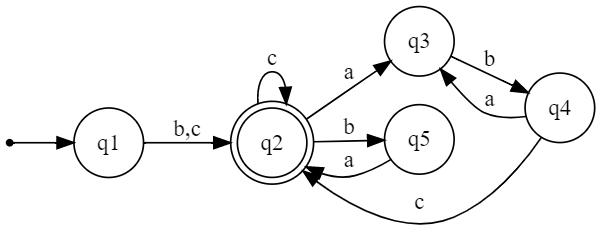
\includegraphics[width=0.6\columnwidth]{3_7.png}
    \end{figure}

Минимизируем его:

\begin{comment}
digraph {
    rankdir="LR"
    "" [shape=point]
    q1 [shape=circle]
    q2 [shape=circle]
    q3 [shape=circle]
    q4 [shape=circle]
    q5 [shape=circle]
    q6q7 [shape=doublecircle]

    "" -> q1
    q1 -> q2 [label="b,c"]
    q2 -> q3 [label="a"]
    q2 -> q4 [label="b"]
    q3 -> q5 [label="b"]
    q5 -> q3 [label="a"]
    q4 -> q6q7 [label="a"]
    q5 -> q6q7 [label="c"]
    q6q7 -> q3 [label="a"]
    q6q7 -> q4 [label="b"]
}
\end{comment}

    \begin{figure}[H]
        \centering
        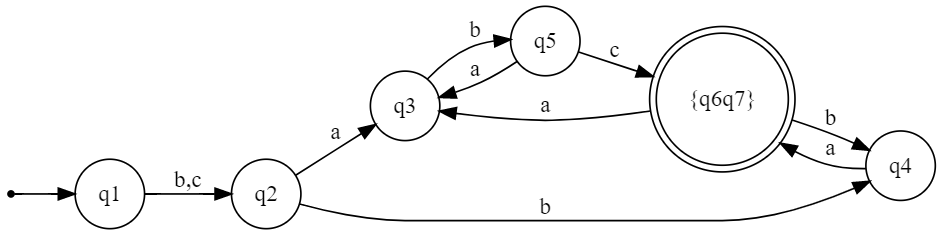
\includegraphics[width=0.6\columnwidth]{3_8.png}
    \end{figure}

%конец 3_4%

%начало 3_5%
    \item \((a+b)^+(aa+bb+abab+baba)(a+b)^+\)
\\Построим НКА:

\begin{comment}
digraph {
    rankdir="LR"
    "" [shape=point]
    q1 [shape=circle]
    q2 [shape=circle]
    q3 [shape=circle]
    q4 [shape=circle]
    q5 [shape=circle]
    q6 [shape=circle]
    q7 [shape=circle]
    q8 [shape=circle]
    q9 [shape=circle]
    q10 [shape=circle]
    q11 [shape=doublecircle]

    "" -> q1
    q1 -> q2 [label="a,b"]
    q2 -> q1 [label="a,b"]
    q2 -> q3 [label="a"]
    q2 -> q4 [label="b"]
    q3 -> q5 [label="b"]
    q3 -> q9 [label="a"]
    q4 -> q6 [label="a"]
    q4 -> q10 [label="b"]
    q5 -> q7 [label="a"]
    q6 -> q8 [label="b"]
    q7 -> q9 [label="b"]
    q8 -> q10 [label="a"]
    q9 -> q11 [label="a,b"]
    q10 -> q11 [label="a,b"]
    q11 -> q11 [label="a,b"]
}
\end{comment}

    \begin{figure}[H]
        \centering
        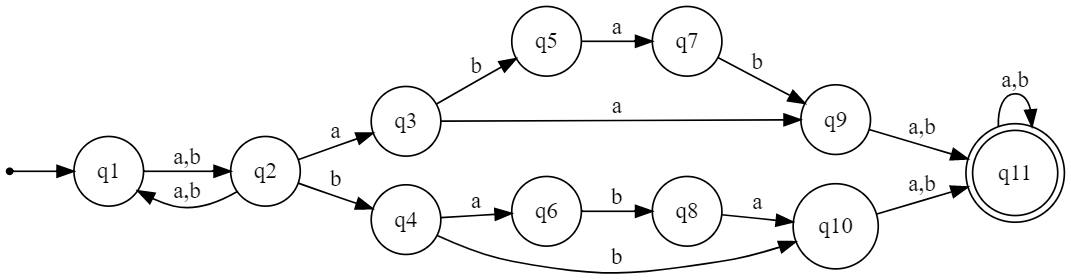
\includegraphics[width=0.6\columnwidth]{3_9.png}
    \end{figure}
 
Преобразуем в ДКА:

\begin{comment}
digraph {
    rankdir="LR"
    "" [shape=point]
    q1 [shape=circle]
    q2 [shape=circle]
    "{q1q3}" [shape=circle]
    "{q2q5}" [shape=circle]
    "{q1q4}" [shape=circle]
    "{q2q6}" [shape=circle]
    "{q1q4q8}" [shape=circle]
    "{q2q6q10}" [shape=circle]
    "{q2q10}" [shape=circle]
    "{q1q3q7}" [shape=circle]
    "{q2q9}" [shape=circle]
    "{q1q3q11}" [shape=doublecircle]
    "{q2q5q11}" [shape=doublecircle]
    "{q2q5q9}" [shape=circle]
    "{q1q3q7q11}" [shape=doublecircle]
    "{q2q9q11}" [shape=doublecircle]
    "{q2q5q9q11}" [shape=doublecircle]
    "{q1q4q11}" [shape=doublecircle]
    "{q2q6q11}" [shape=doublecircle]
    "{q1q4q8q11}" [shape=doublecircle]
    "{q2q6q10q11}" [shape=doublecircle]
    "{q2q10q11}" [shape=doublecircle]

    "" -> q1
    q1 -> q2 [label="a, b"]
    q2 -> "{q1q3}" [label="a"]
    q2 -> "{q1q4}" [label="b"]
    "{q1q3}" -> "{q2q9}" [label="a"]
    "{q1q3}" -> "{q2q5}" [label="b"]
    "{q2q5}" -> "{q1q3q7}" [label="a"]
    "{q2q5}" -> "{q1q4}" [label="b"]
    "{q1q4}" -> "{q2q6}" [label="a"]
    "{q1q4}" -> "{q2q10}" [label="b"]
    "{q2q6}" -> "{q1q3}" [label="a"]
    "{q2q6}" -> "{q1q4q8}" [label="b"]
    "{q1q4q8}" -> "{q2q6q10}" [label="a"]
    "{q1q4q8}" -> "{q2q10}" [label="b"]
    "{q2q6q10}" -> "{q1q3q11}" [label="a"]
    "{q2q6q10}" -> "{q1q4q8q11}" [label="b"]
    "{q2q10}" -> "{q1q3q11}" [label="a"]
    "{q2q10}" -> "{q1q4q11}" [label="b"]
    "{q1q3q7}" -> "{q2q9}" [label="a"]
    "{q1q3q7}" -> "{q2q5q9}" [label="b"]
    "{q2q9}" -> "{q1q3q11}" [label="a"]
    "{q2q9}" -> "{q1q4q11}" [label="b"]
    "{q1q3q11}" -> "{q2q9q11}" [label="a"]
    "{q1q3q11}" -> "{q2q5q11}" [label="b"]
    "{q2q5q11}" -> "{q1q3q7q11}" [label="a"]
    "{q2q5q11}" -> "{q1q4q11}" [label="b"]
    "{q2q5q9}" -> "{q1q4q11}" [label="b"]
    "{q2q5q9}" -> "{q1q3q7q11}" [label="a"]
    "{q2q5q9}" -> "{q1q4q11}" [label="b"]
    "{q1q3q7q11}" -> "{q2q9q11}" [label="a"]
    "{q1q3q7q11}" -> "{q2q5q9q11}" [label="b"]
    "{q2q9q11}" -> "{q1q4q11}" [label="b"]
    "{q2q5q9q11}" -> "{q1q3q7q11}" [label="a"]
    "{q2q5q9q11}" -> "{q1q4q11}" [label="b"]
    "{q1q4q11}" -> "{q2q6q11}" [label="a"]
    "{q1q4q11}" -> "{q2q10q11}" [label="b"]
    "{q2q6q11}" -> "{q1q4q8q11}" [label="b"]
    "{q1q4q8q11}" -> "{q2q6q10q11}" [label="a"]
    "{q1q4q8q11}" -> "{q2q10q11}" [label="b"]
    "{q2q6q10q11}" -> "{q1q3q11}" [label="a"]
    "{q2q6q10q11}" -> "{q1q4q8q11}" [label="b"]
    "{q2q10q11}" -> "{q1q3q11}" [label="a"]
    "{q2q10q11}" -> "{q1q4q11}" [label="b"]
}
\end{comment}

    \begin{figure}[H]
        \centering
        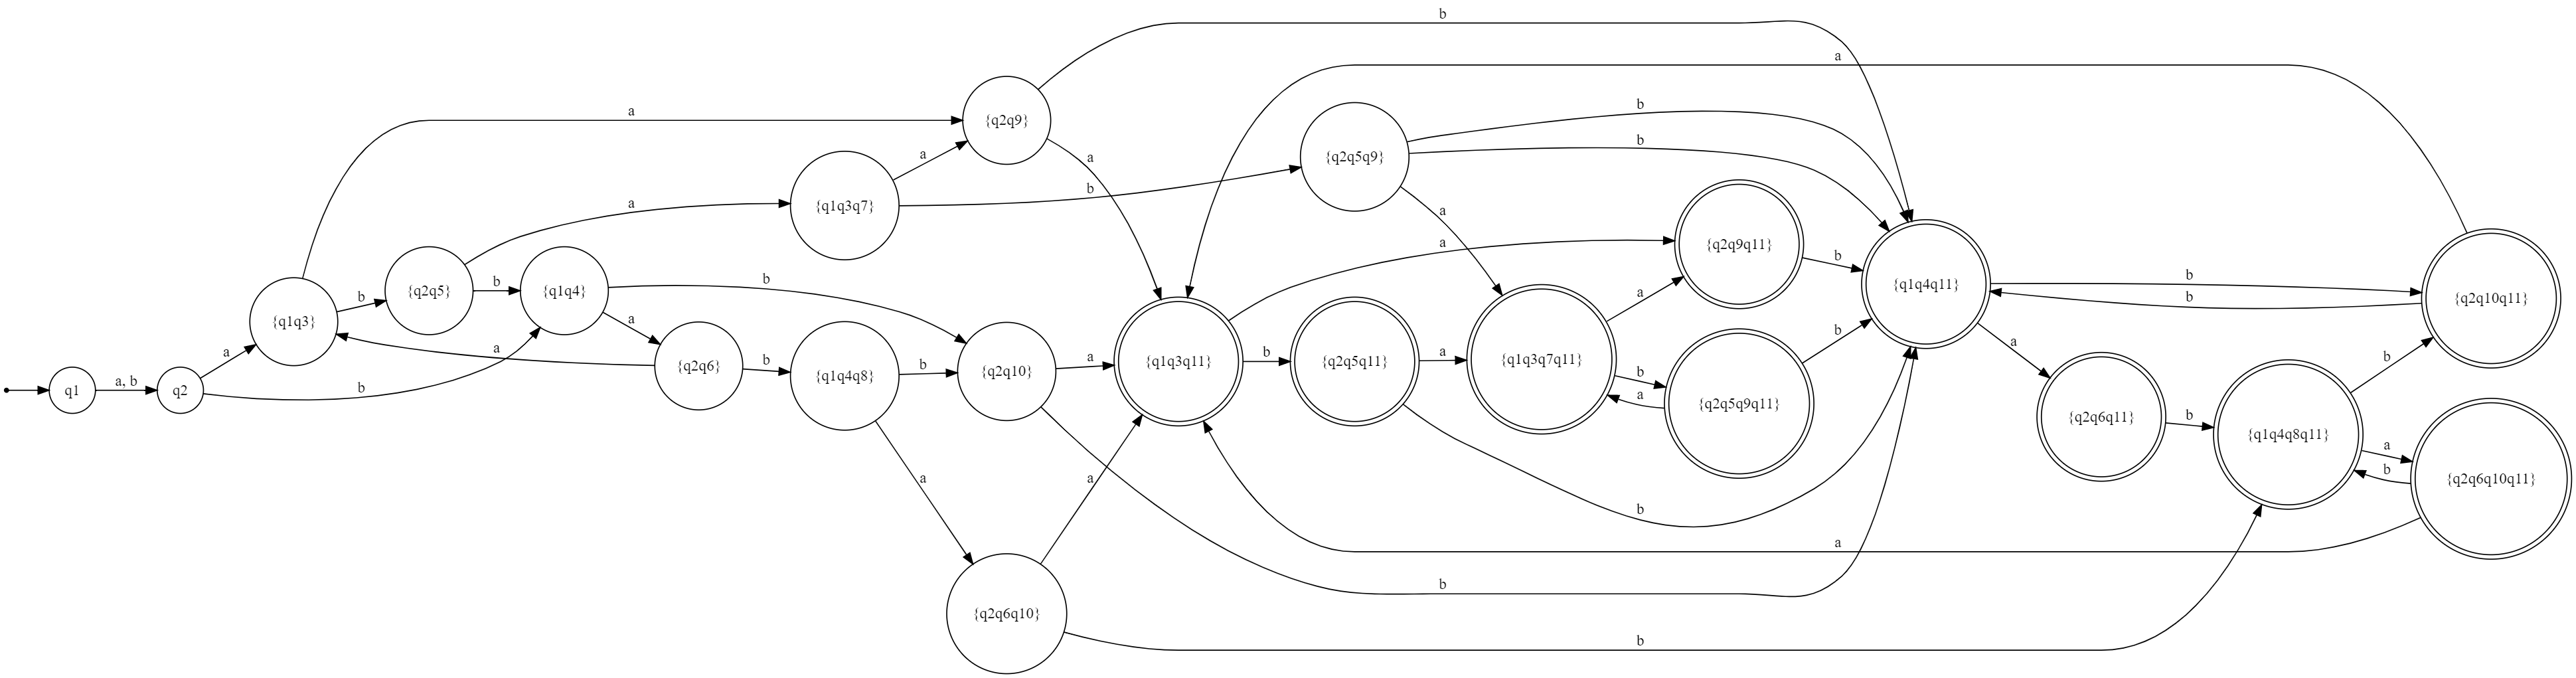
\includegraphics[width=1\columnwidth]{3_10.png}
    \end{figure}

Минимизируем ДКА и переобозначим эквивалентные вершины:
\begin{itemize}
    \item q1 - Q1
    \item q2 - Q2
    \item {q1q3} - Q3
    \item {q1q4} - Q4
    \item {q2q5} - Q5
    \item {q2q6} - Q6
    \item {q1q3q7}, {q1q4q8} - Q7
    \item {q2q9}, {q2q6q10}, {q2q5q9}, {q2q10} - Q8
    \item {q2q5q11}, {q1q3q11}, {q2q6q1011}, {q2q6q11}, {q1q4q8q11}, {q1q4q11}, {q2q10q11}, {q1q3q7q11}, {q2q9q11}, {q2q5q9q11} - Q9
\end{itemize}

\begin{comment}
digraph {
    rankdir="LR"
    "" [shape=point]
    Q1 [shape=circle]
    Q2 [shape=circle]
    Q3 [shape=circle]
    Q4 [shape=circle]
    Q5 [shape=circle]
    Q6 [shape=circle]
    Q7 [shape=circle]
    Q8 [shape=circle]
    Q9 [shape=doublecircle]

    "" -> Q1
    Q1 -> Q2 [label="a, b"]
    Q2 -> Q3 [label="a"]
    Q2 -> Q4 [label="b"]
    Q3 -> Q8 [label="a"]
    Q3 -> Q5 [label="b"]
    Q4 -> Q6 [label="a"]
    Q4 -> Q8 [label="b"]
    Q5 -> Q7 [label="a"]
    Q5 -> Q4 [label="b"]
    Q6 -> Q3 [label="a"]
    Q6 -> Q7 [label="b"]
    Q7 -> Q8 [label="a,b"]
    Q8 -> Q9 [label="a,b"]
    Q9 -> Q9 [label="a,b"]
}
\end{comment}

    \begin{figure}[H]
        \centering
        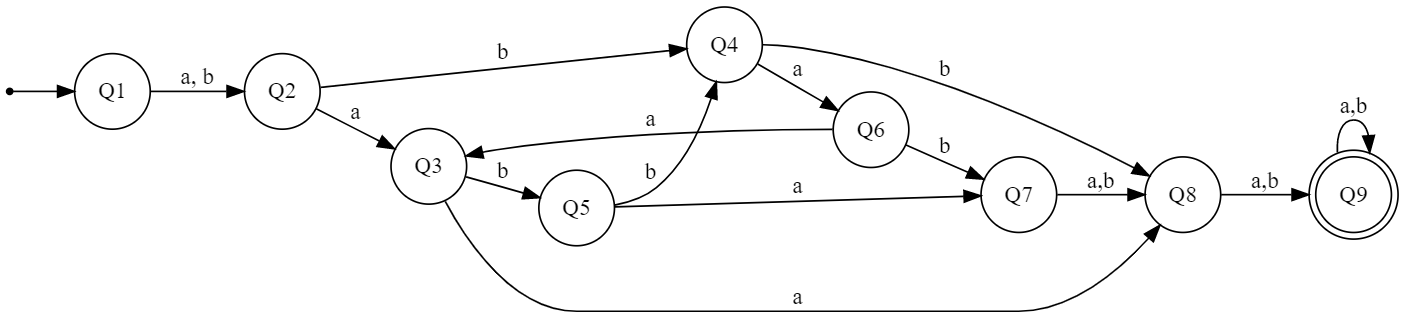
\includegraphics[width=1\columnwidth]{3_11.png}
    \end{figure}

%конец 3_5%
\end{enumerate}

%часть 4%
\section{Задание №4. Построить минимальный ДКА по регулярному выражению.}
Ответом на данное задание является минимальный ДКА, который допускает тот же язык, что описывается регулярным выражением.
\begin{enumerate}
%начало 4_1%
    \item \(L=\{(aab)^n(aba)^m | n \geq 0, m \geq 0\} \)
\\Конечный автомат, распознающий данный язык:

\begin{comment}
digraph {
    rankdir="LR"
    "" [shape=point]
    q1 [shape=circle]
    q2 [shape=doublecircle]
    q3 [shape=circle]
    q4 [shape=circle]
    q5 [shape=circle]
    q6 [shape=circle]

    "" -> q1
    q1 -> q2 [label="b"]
    q1 -> q3 [label="a"]
    q3 -> q4 [label="a"]
    q4 -> q1 [label="b"]
    q2 -> q5 [label="a"]
    q5 -> q6 [label="b"]
    q6 -> q2 [label="a"]
}
\end{comment}

    \begin{figure}[H]
        \centering
        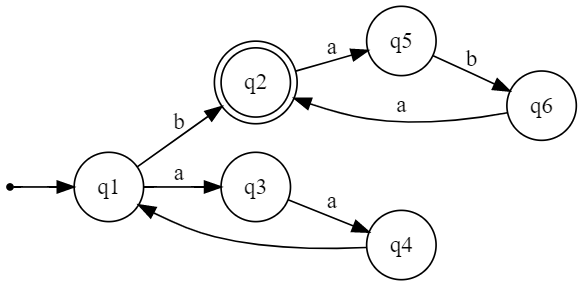
\includegraphics[width=0.6\columnwidth]{4_1.png}
    \end{figure}
Соответственно, язык является регулярным.
%конец 4_1%

%начало 4_2%
    \item \(L=\{uaav | u \in \{a,b\}^*, v \in \{a,b\}^*, |u|_b \geq |v|_a\}\)
\\Воспользуемся леммой о разрастании.
\\Зафиксируем \(\forall n \in \mathbb{N}\) и рассмотрим слово \(\omega = b^naaa^n, |\omega|=2n+2 \geq n\).
\begin{center}
\(\omega = xyz, |y| \neq 0, |xy| \leq n:\)
\\\(x=b^m, y=b^l, z=b^{n-m-l}aaa^n\)
\\\(m+l \leq n, l \neq 0\)
\\\(\omega = xy^kz=b^mb^{il}b^{n-m-l}aaa^n\)
\\Пусть i=0, тогда: \(\omega = b^{n-l}aaa^n \notin L, l \neq 0\)
\end{center}
Лемма не выполняется. Делаем вывод, что язык не является регулярным.
%конец 4_2%

%начало 4_3%
    \item \(L=\{a^m\omega | \omega \in \{a,b\}^*, 1 \leq |\omega|_b \leq m\}\)
\\Воспользуемся леммой о разрастании.
\\Зафиксируем \(\forall n \in \mathbb{N}\) и рассмотрим слово \(\omega = a^nb^n, |\omega|=2n \geq n\).
\begin{center}
\(\omega = xyz, |y| \neq 0, |xy| \leq n:\)
\\\(x=a^m, y=a^l, z=a^{n-m-l}b^n\)
\\\(m+l \leq n, l \neq 0\)
\\\(\omega = xy^kz=a^ma^{il}a^{n-m-l}b^n\)
\\Пусть i=0, тогда: \(\omega = a^{n-l}b^n \notin L, l \neq 0\)
\end{center}
Лемма не выполняется. Делаем вывод, что язык не является регулярным.
%конец 4_3%

%начало 4_4%
    \item \(L=\{a^kb^ma^n | k = n \vee m > 0\}\)
\\Воспользуемся леммой о разрастании.
\\Зафиксируем \(\forall n \in \mathbb{N}\) и рассмотрим слово \(\omega = a^nba^n, |\omega|=2n+1 \geq n\).
\begin{center}
\(\omega = xyz, |y| \neq 0, |xy| \leq n:\)
\\\(x=a^m, y=a^l, z=a^{n-m-l}ba^n\)
\\\(m+l \leq n, l \neq 0\)
\\\(\omega = xy^iz=a^ma^{il}a^{n-m-l}ba^n\)
\\Пусть i=2, тогда: \(\omega = a^{n+l}ba^n \notin L, l \neq 0\)
\end{center}
Лемма не выполняется. Делаем вывод, что язык не является регулярным.
%конец 4_4%

%начало 4_5%
    \item \(L=\{ucv | u \in \{a,b\}^*, v \in \{a,b\}^*, u \neq v^R\}\)
\\Воспользуемся леммой о разрастании.
\\Зафиксируем \(\forall n \in \mathbb{N}\) и рассмотрим слово \(\omega = (ab)^nc(ab)^n=\alpha_1\alpha_2...\alpha_n...\alpha_{2n}...\alpha_{4n}\alpha_{4n+1}, |\omega|=4n+1 \geq n\).
\begin{center}
\(\omega = xyz, |y| \neq 0, |xy| \leq n:\)
\\\(x=\alpha_1\alpha_2...\alpha_m, y=\alpha_{m+1}\alpha_{m+2}...\alpha_{m+l}, z=\alpha_{m+l+1}\alpha_{m+l+2}...\alpha_{4n+1}c(ab)^n\)
\\\(m+l \leq n, l \neq 0\)
\\\(\omega = xy^iz=(\alpha_1\alpha_2...\alpha_m)(\alpha_{m+1}\alpha_{m+2}...\alpha_{m+l})^i,(\alpha_{m+l+1}\alpha_{m+l+2}...\alpha_{4n+1}c(ab)^n)\)
\\Пусть i=2, тогда: \(\omega = (\alpha_1\alpha_2...\alpha_m)(\alpha_{m+1}\alpha_{m+2}...\alpha_{m+l})^2,(\alpha_{m+l+1}\alpha_{m+l+2}...\alpha_{4n+1}c(ab)^n) \notin L, l \neq 0\)
\end{center}
Лемма не выполняется. Делаем вывод, что язык не является регулярным.
%конец 4_5%
\end{enumerate}
\end{document}


